% Question 1-12
\section{}\label{sec:1}
In order to generate the heat maps of two reward functions, we construct the \verb"plot-heatmap" function using \verb"pcolor" from \verb"matplotlib". Figure \ref{fig: heatmap1} shows the heat maps for reward function 1 and 2.

\begin{figure}[!htb]
\centering
  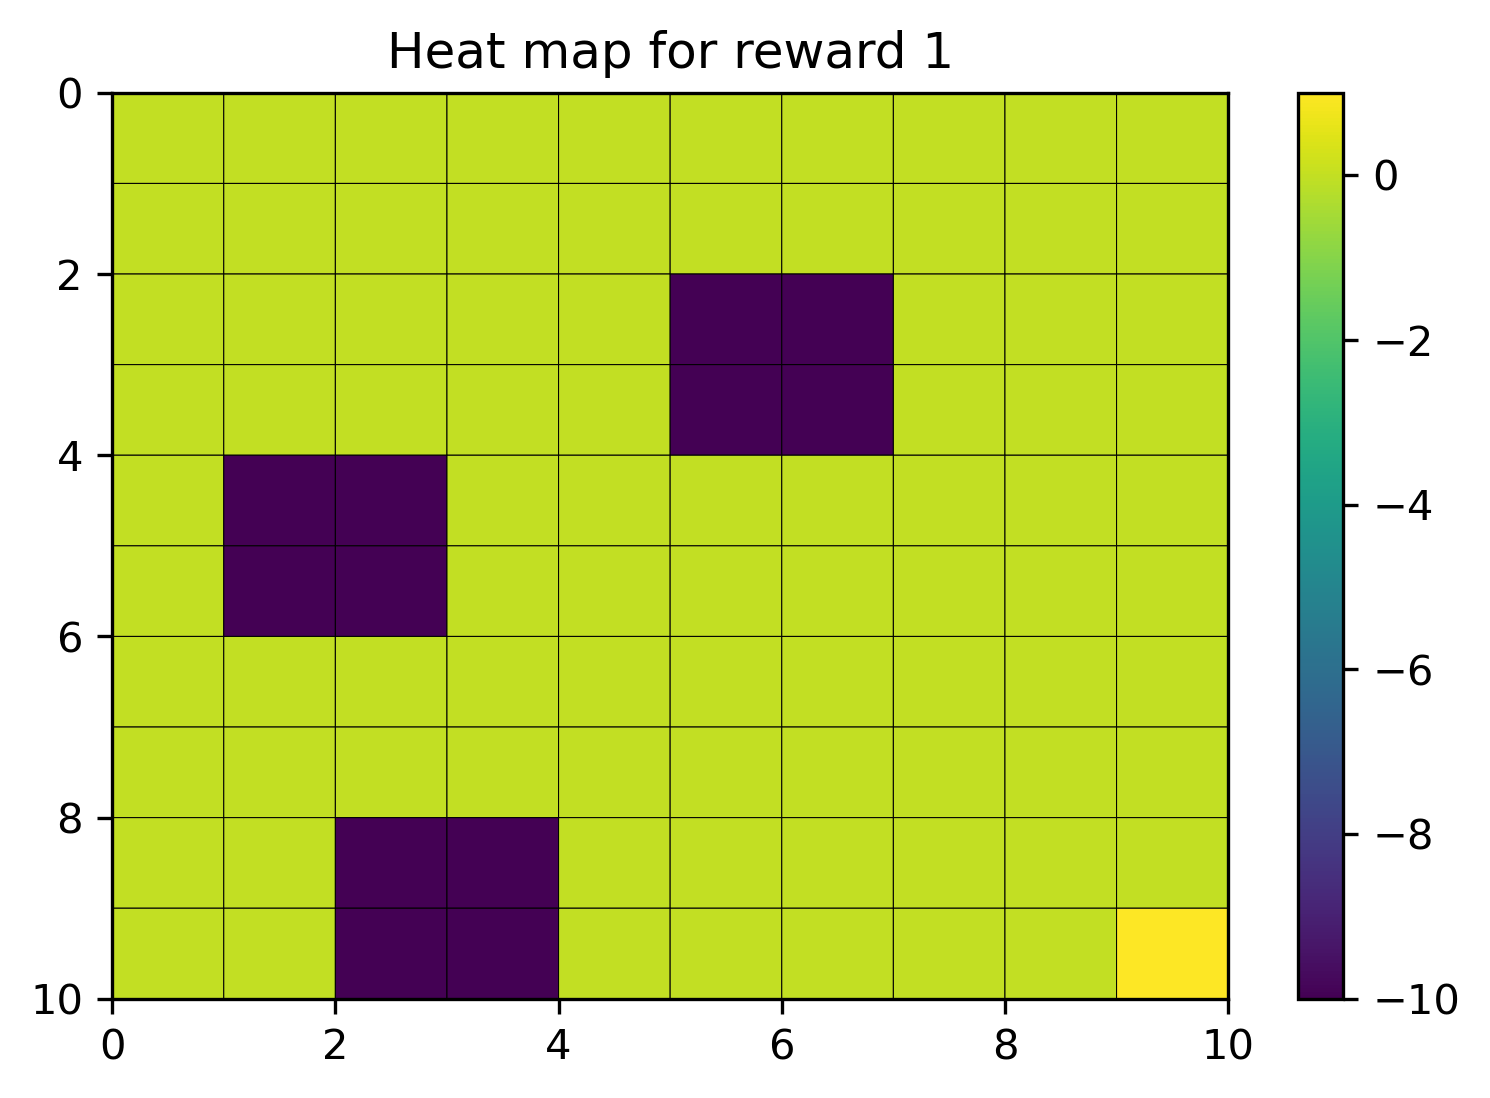
\includegraphics[width=0.49\textwidth]{images/Q1-9/Heat-map-for-reward-1.png}
  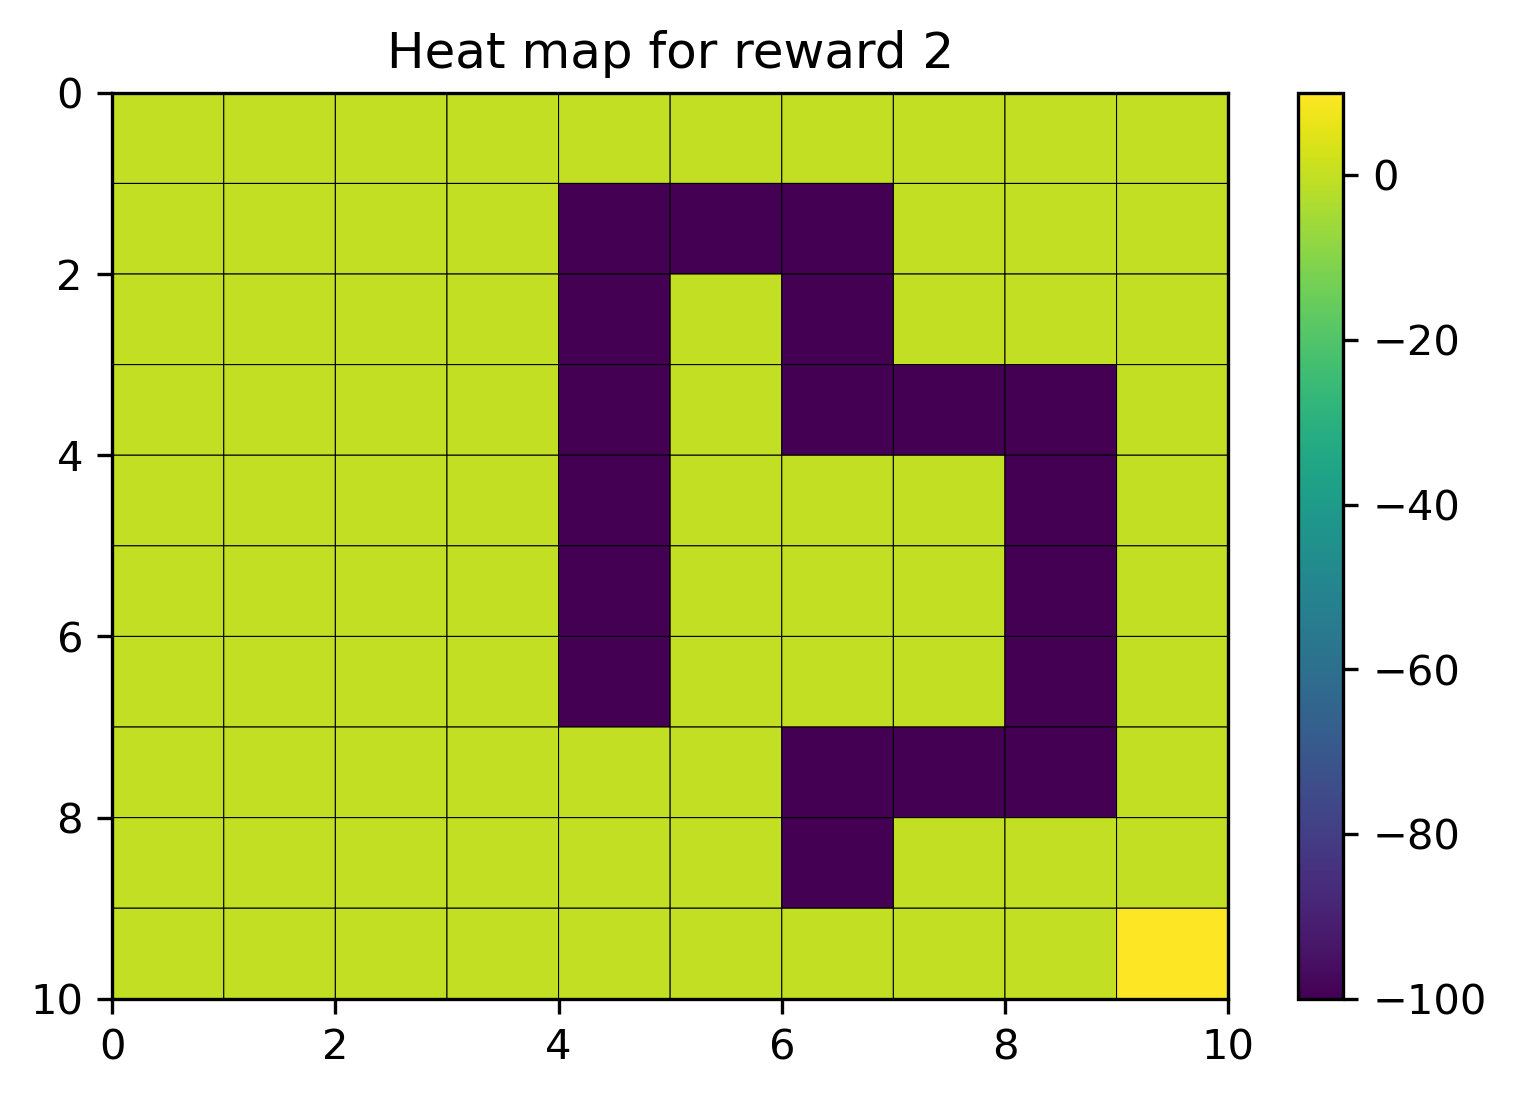
\includegraphics[width=0.49\textwidth]{images/Q1-9/Heat-map-for-reward-2.png}
  \caption{Heatmap for ground-truth reward functions}
\label{fig: heatmap1}
\end{figure}

\section{}\label{sec:2}
We first create the MDP class called \verb"gridworld" which include environment information: 10 grid size and $|S|=10^2$ possible states; 4 possible actions; wind probability $w=0.1$. We use a private function within the class to calculate the transition probability matrix $\mathcal{P}_{s s^{\prime}}^a$. For each action and starting state, we calculate the probability to the possible next states $\mathcal{P}_s^a \in \mathbb{R}^{|S|\times1}$. We do this by adding $w/4$ to all directions (for directions that goes off-grid, the probability simply accumulate on the starting state) and then add $1-w$ on the intended direction.

We then create the \verb"value_iteration" function to implement the value iteration algorithm. It takes the gridworld object and a reward function as input, along with the parameters given in the project: discount factor $\gamma=0.8$ and threshold for convergence $\Delta\leqslant\epsilon=0.01$. There are three outputs from the \verb"value_iteration" function: the optimal state value function $V(s)\in \mathbb{R}^{|S|\times1}$; the optimal policy $\pi (s)\in \mathbb{R}^{|S|\times1}$; and the converging iterations $N$. We also create functions to plot our results.

We instantiate a gridworld object and start our simulation. Using result function 1, the value iteration converges in $N=21$ steps. We show the snapshots of the state value function for step 1, 5, 9, 13, 17, 21 in Figure \ref{fig: matrix1}. It can been observed from the figure that: 
\begin{itemize}
    \item The final optimal state values reach to the maximum and minimum on the same states as the reward function. The larger the reward on a state, the larger the optimal value.
    \item  All states have an initial value 0, the effect of the reward function spreads from non-zero reward states to the whole state space through iterations. 
    \newpage
    \item The increasing speed of the state values depends on two factors: the absolute value of the reward and the number of iterations. A reward closer to 0 and an iteration number closer to convergence lead to low increasing speed.
\end{itemize}


\begin{figure}[!htb]
\centering
  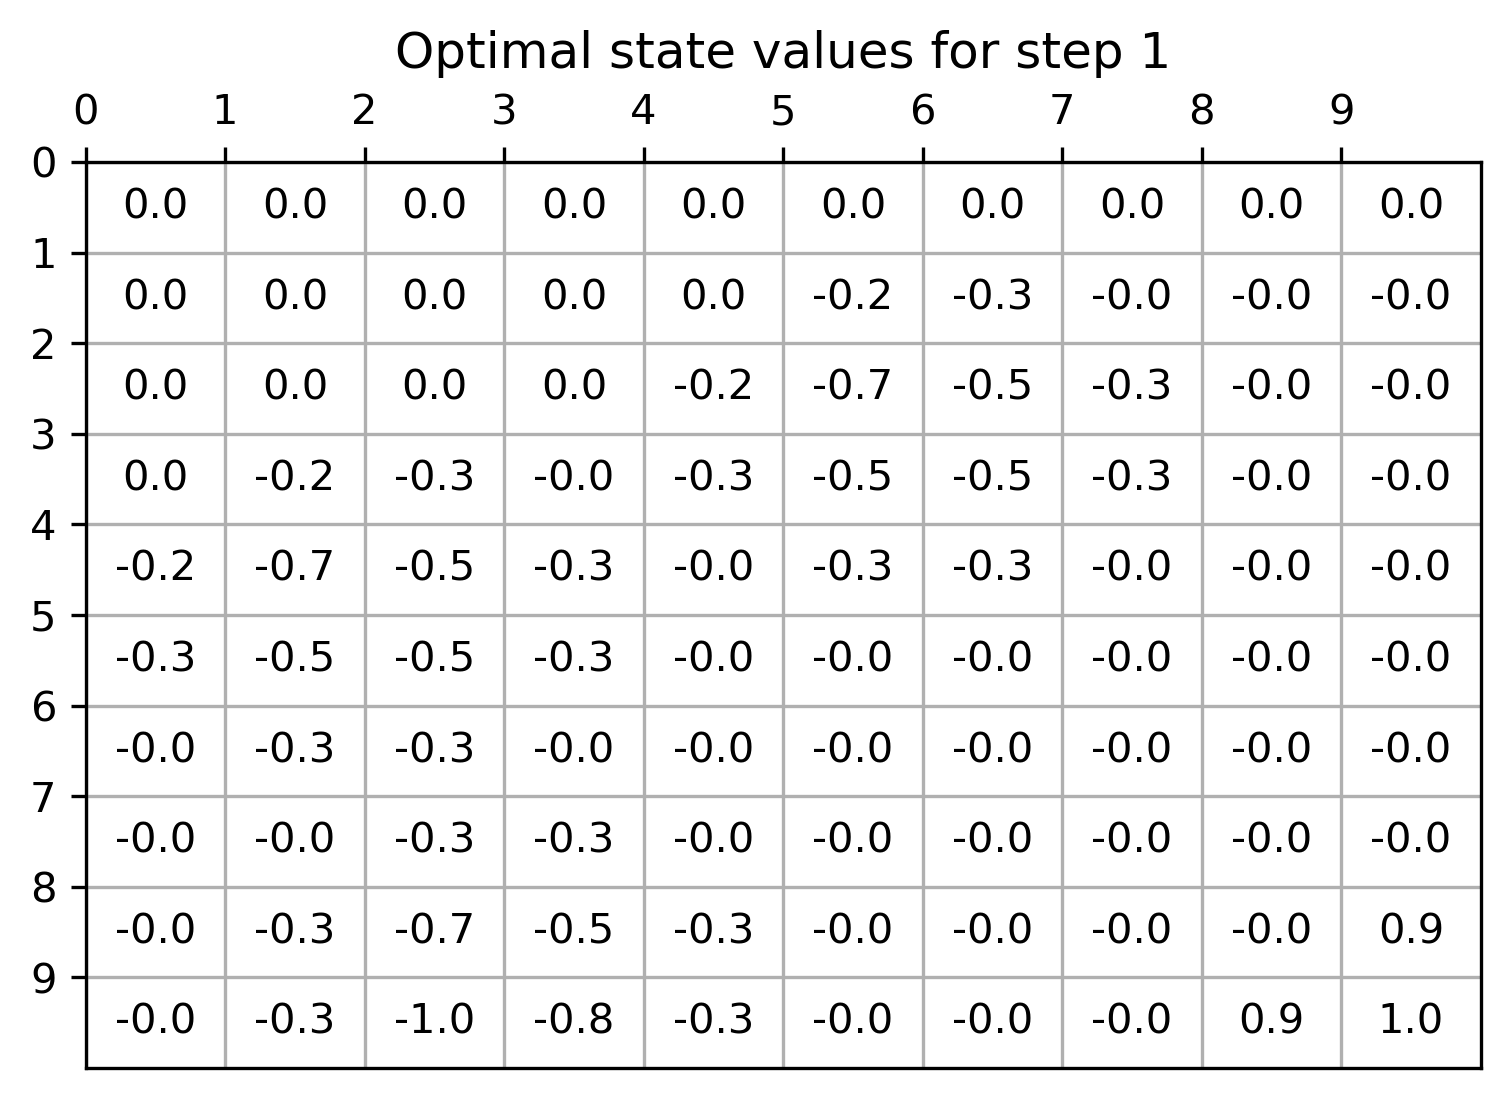
\includegraphics[width=0.49\textwidth]{images/Q1-9/Optimal-state-values-for-step-1.png}
  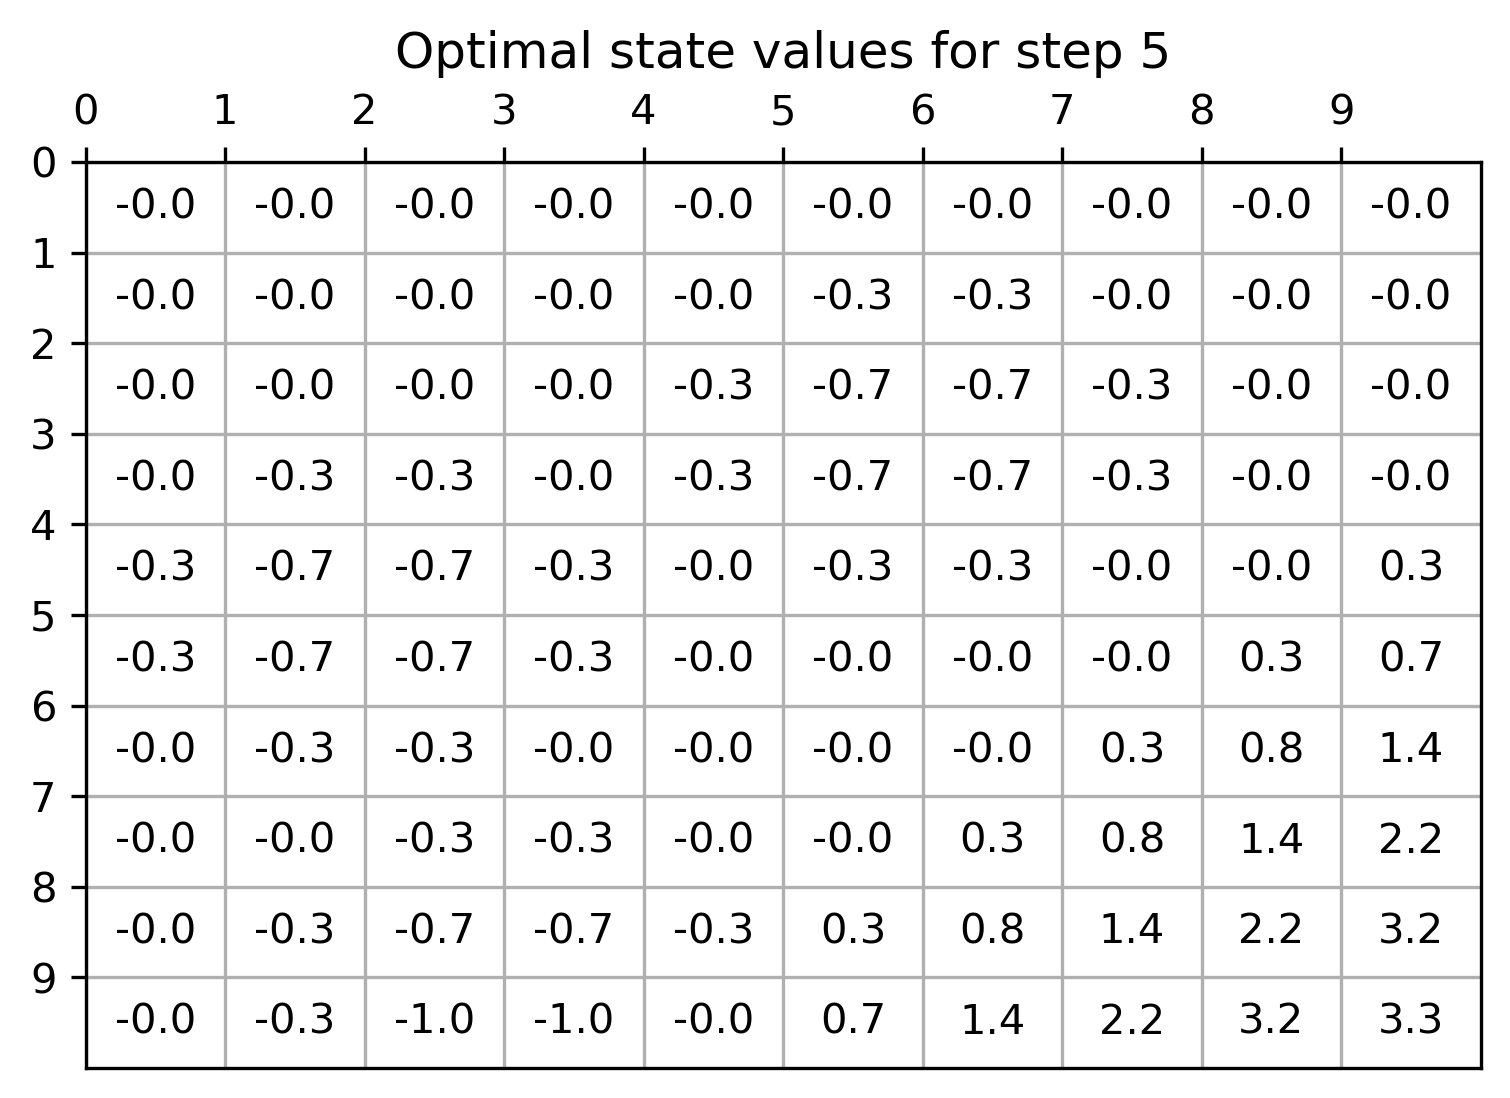
\includegraphics[width=0.49\textwidth]{images/Q1-9/Optimal-state-values-for-step-5.png}
  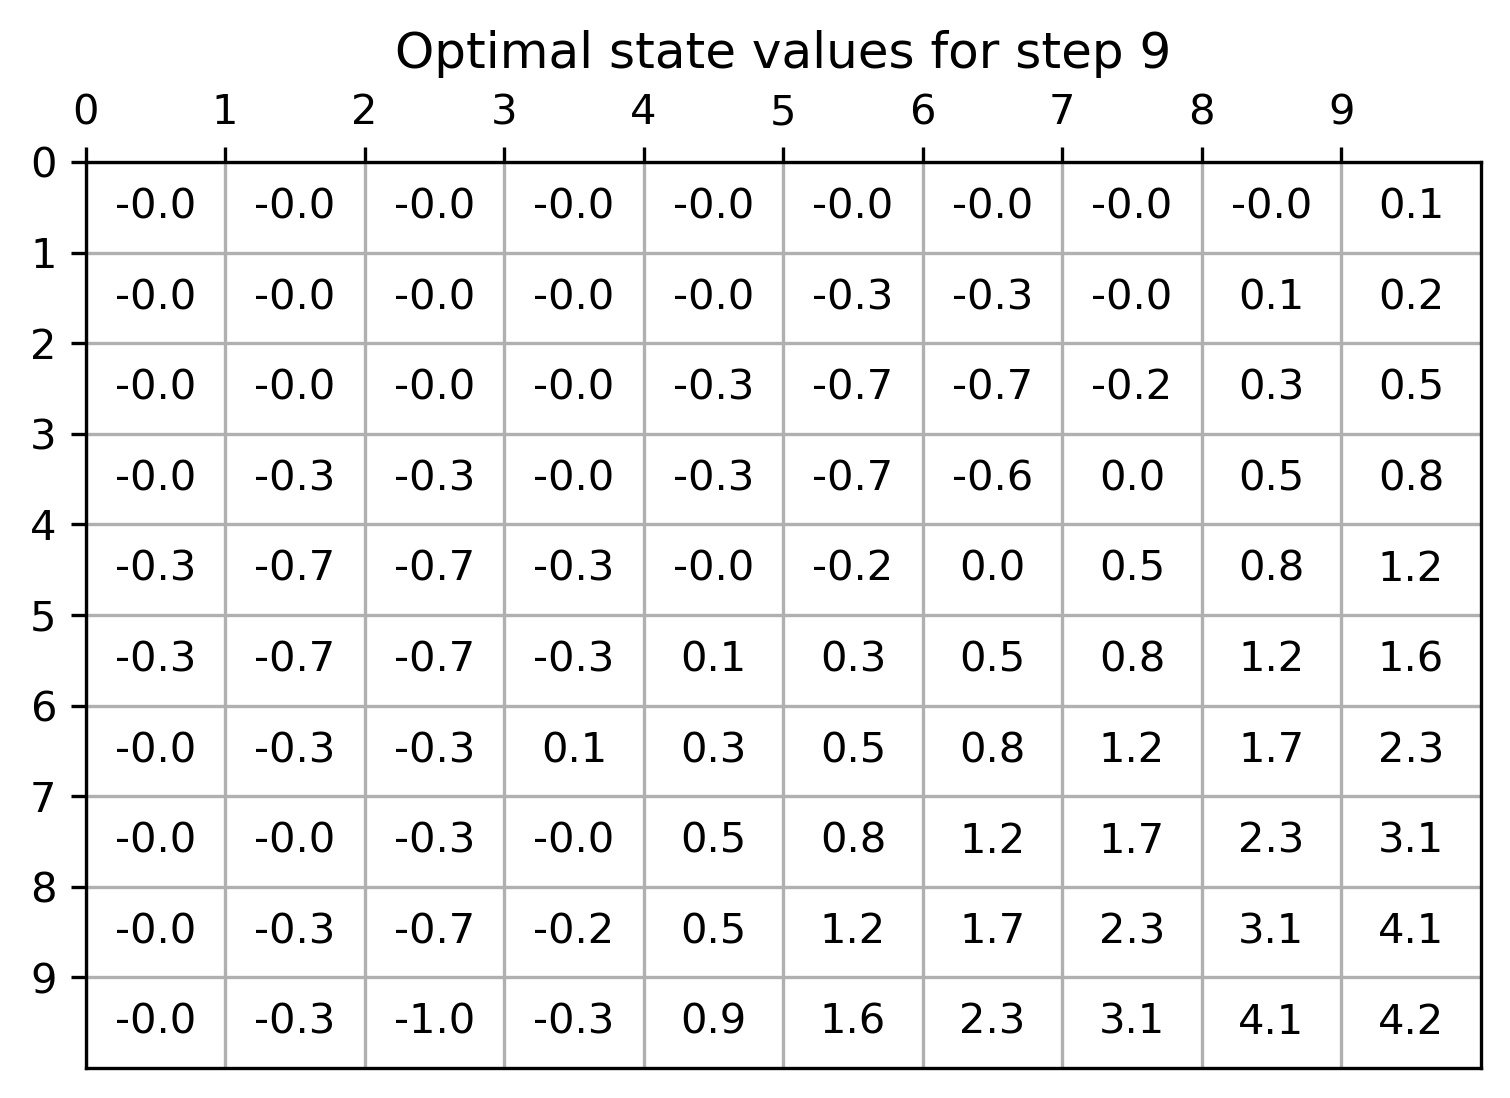
\includegraphics[width=0.49\textwidth]{images/Q1-9/Optimal-state-values-for-step-9.png}
  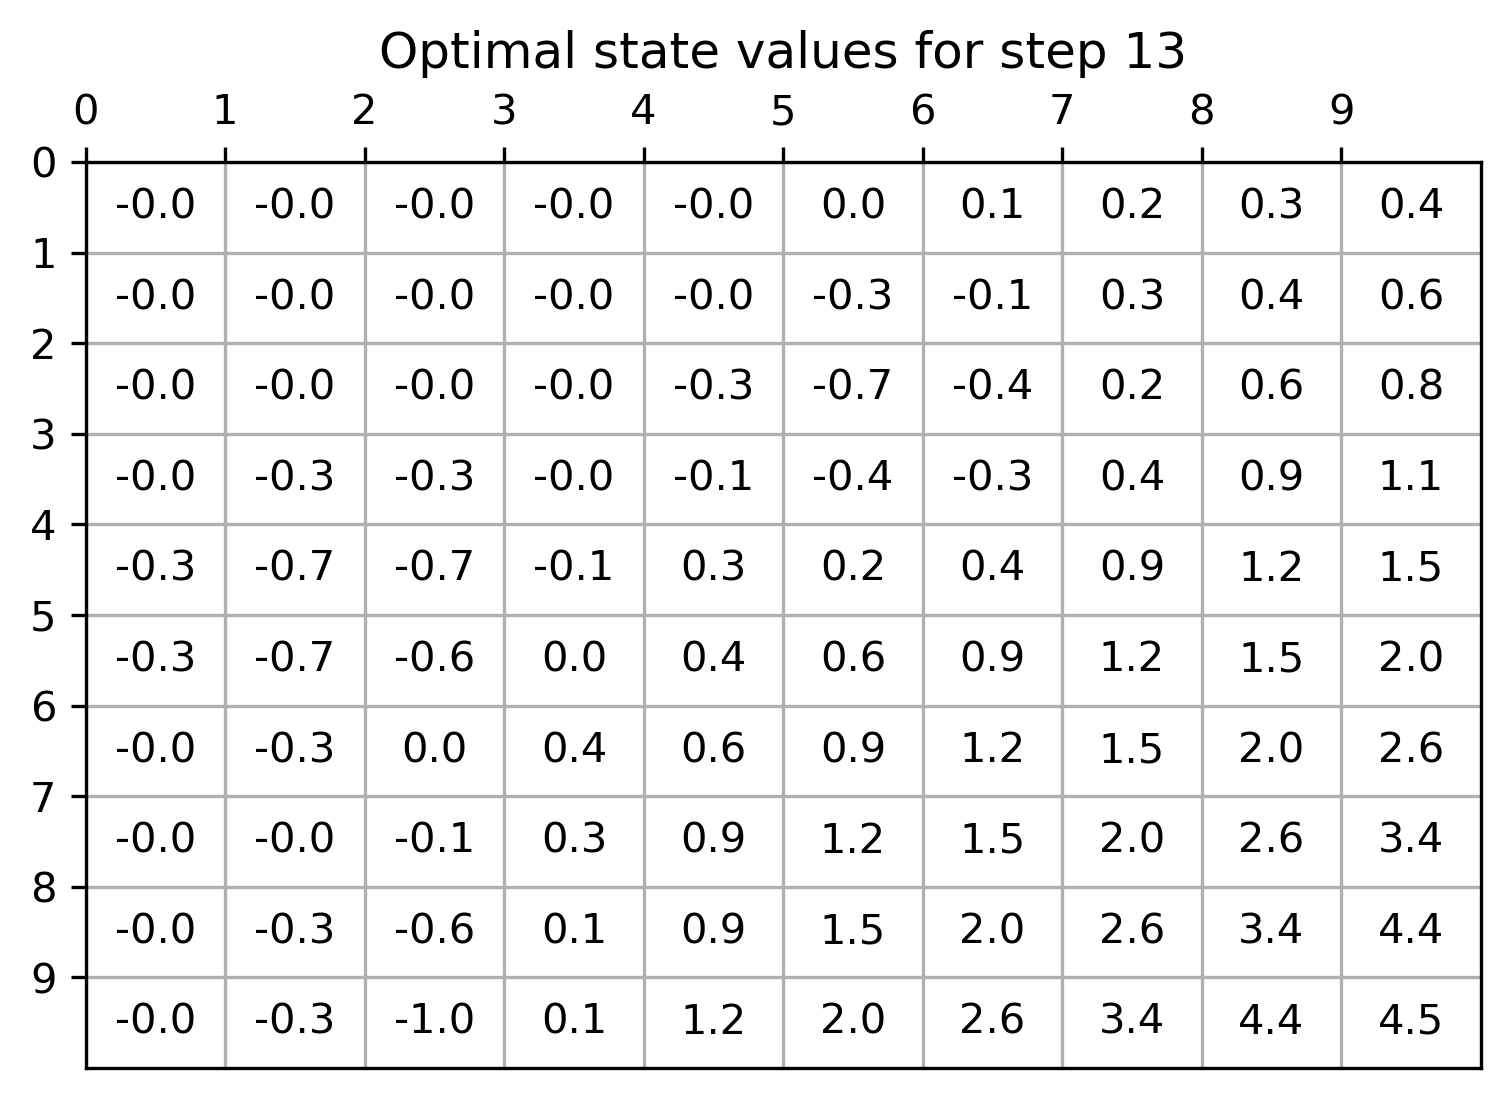
\includegraphics[width=0.49\textwidth]{images/Q1-9/Optimal-state-values-for-step-13.png}
  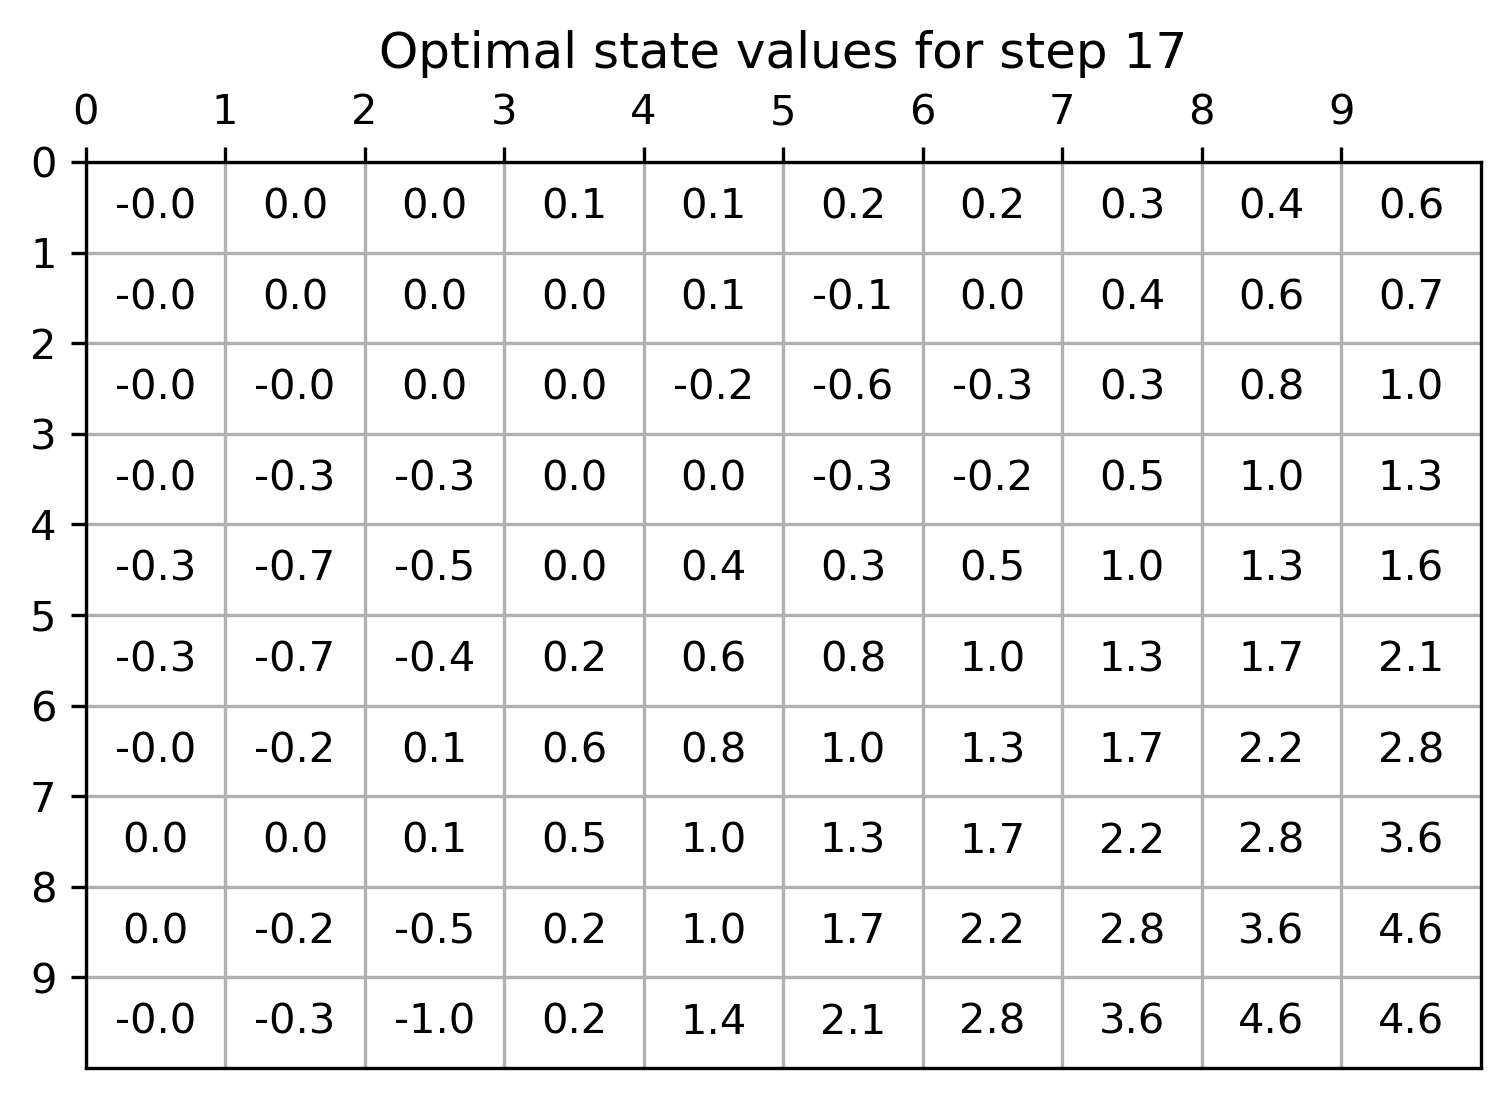
\includegraphics[width=0.49\textwidth]{images/Q1-9/Optimal-state-values-for-step-17.png}
  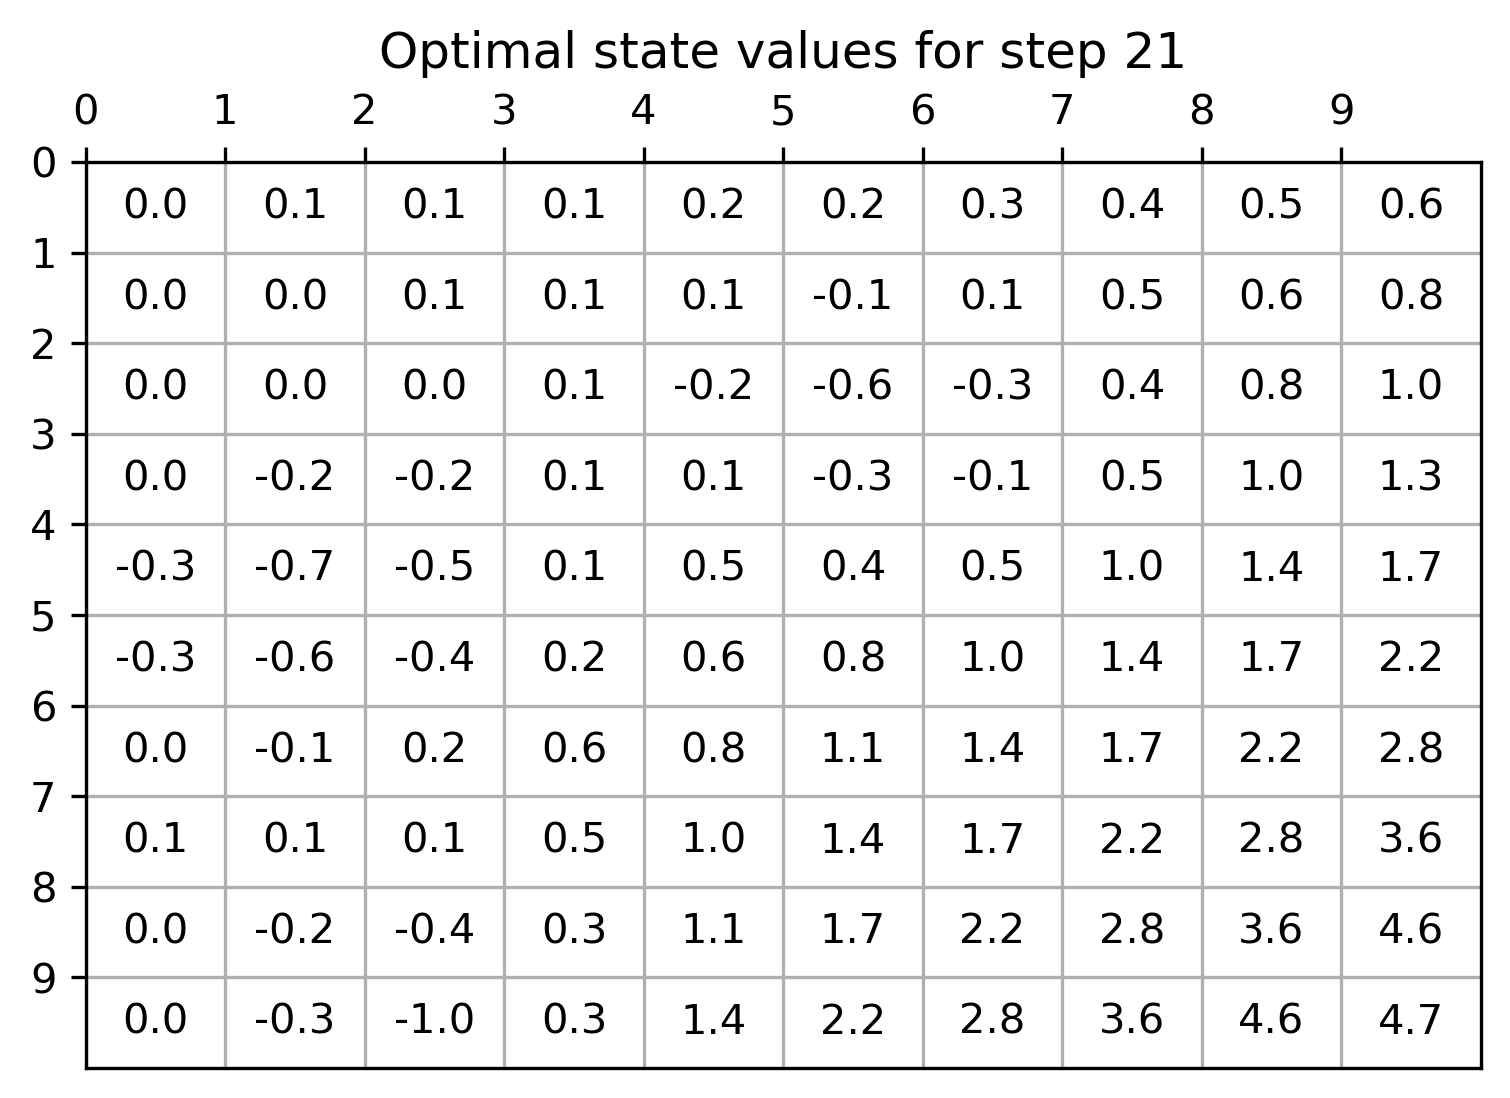
\includegraphics[width=0.49\textwidth]{images/Q1-9/Optimal-state-values-for-step-21.png}
  \caption{Optimal state values for reward 1}
\label{fig: matrix1}
\end{figure}

\section{}\label{sec:3}
Figure \ref{fig: heatmap2} shows the heatmap of the optimal state value function for reward function 1.

\begin{figure}[!htb]
\centering
  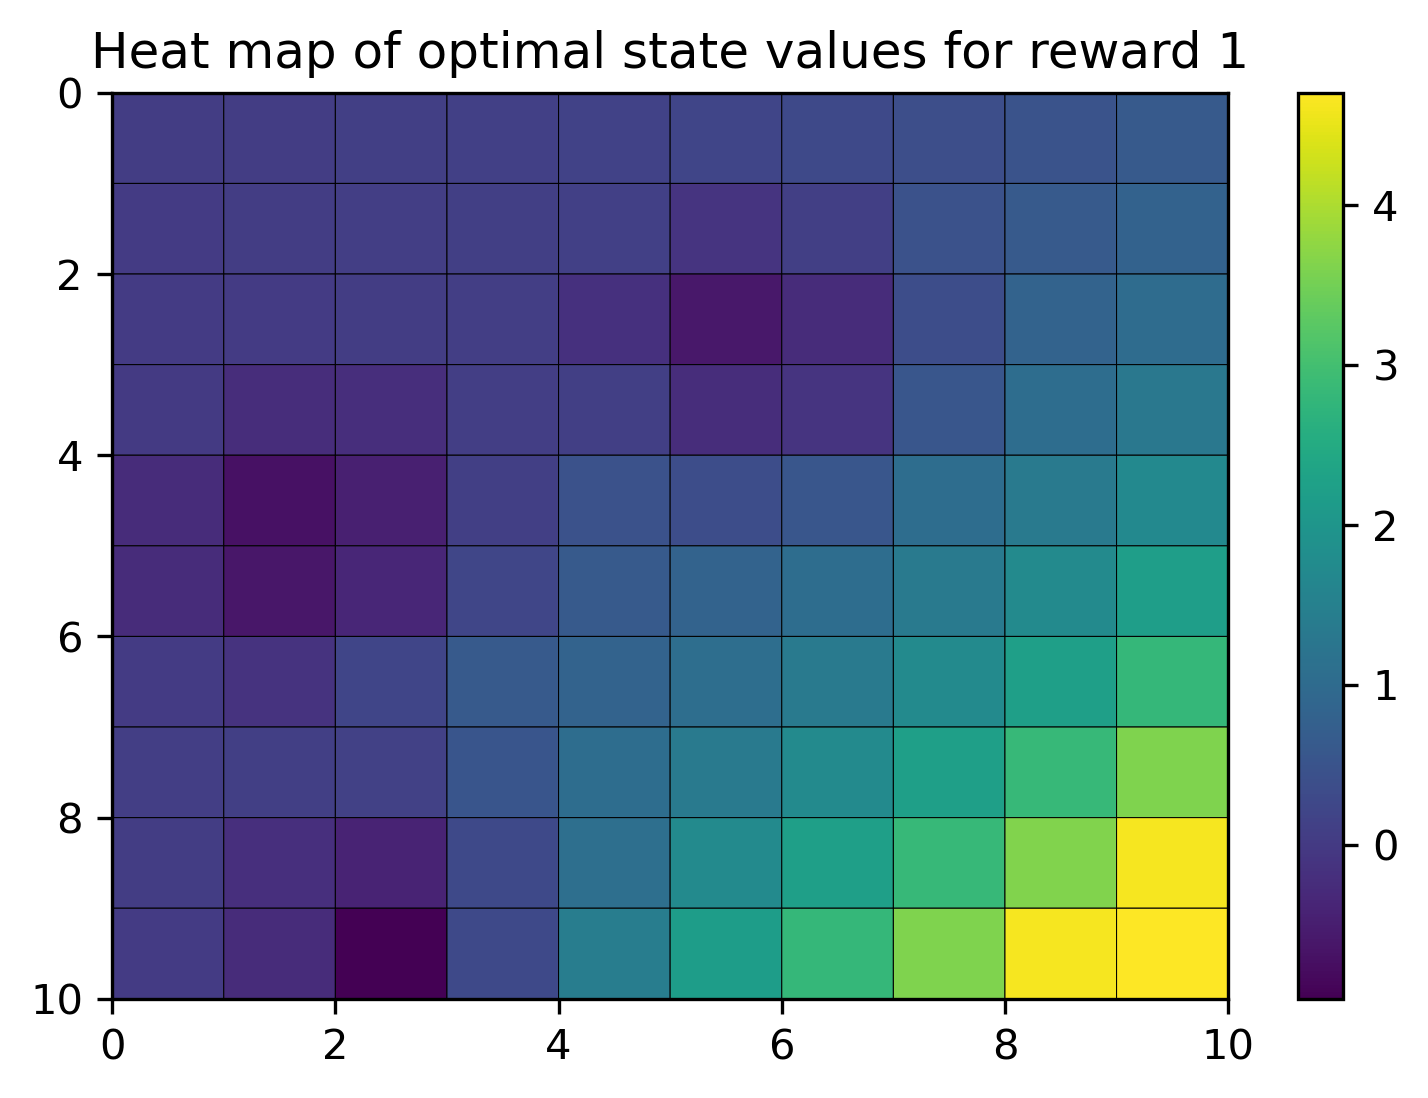
\includegraphics[width=0.49\textwidth]{images/Q1-9/Heat-map-of-optimal-state-values-for-reward-1.png}
  \caption{Heatmap of optimal state value function for reward 1}
\label{fig: heatmap2}
\end{figure}

\section{}\label{sec:4}
Recall the equation to calculate optimal state value function:  

\begin{equation}
\label{eq: optimal-value}
     \begin{aligned} 
         V^{*}(s) 
         &=\max _{a \in \mathcal{A}} Q^{\pi^{*}}(s, a) \\ 
         &=\max _{a \in \mathcal{A}} \mathbb{E}_{\pi^{*}}\left[\sum_{k=0}^{\infty} \gamma^{k} r_{t+k+1} \mid s_{t}=s, a_{t}=a\right] \\
         &=\max _{a \in \mathcal{A}} \sum_{s^{\prime}} \mathcal{P}_{s s^{\prime}}^{a}\left[\mathcal{R}_{s s^{\prime}}^{a}+\gamma V^{*}\left(s^{\prime}\right)\right] \end{aligned}
\end{equation}

We can see that the optimal state value distribution matches the equation in the following aspects:

\begin{itemize}
    \item The optimal value of a state is loosely proportional to its reward. It is not strictly proportional since the optimal value is also affected by the rewards of the other states which propagate to the whole plane.
    \item A visible progressive transition can be observed in the heatmap. This is due to the discount factor $\gamma=0.8$ which prioritize immediate reward over future rewards.
    \item As the value function converges, adjacent state values have less gap with each other, smoothing out the whole 2D grid.
\end{itemize}
\newpage

\section{}\label{sec:5}
Figure \ref{fig: policy1} shows the optimal policy of the agent for reward 1.

\begin{figure}[!htb]
\centering
  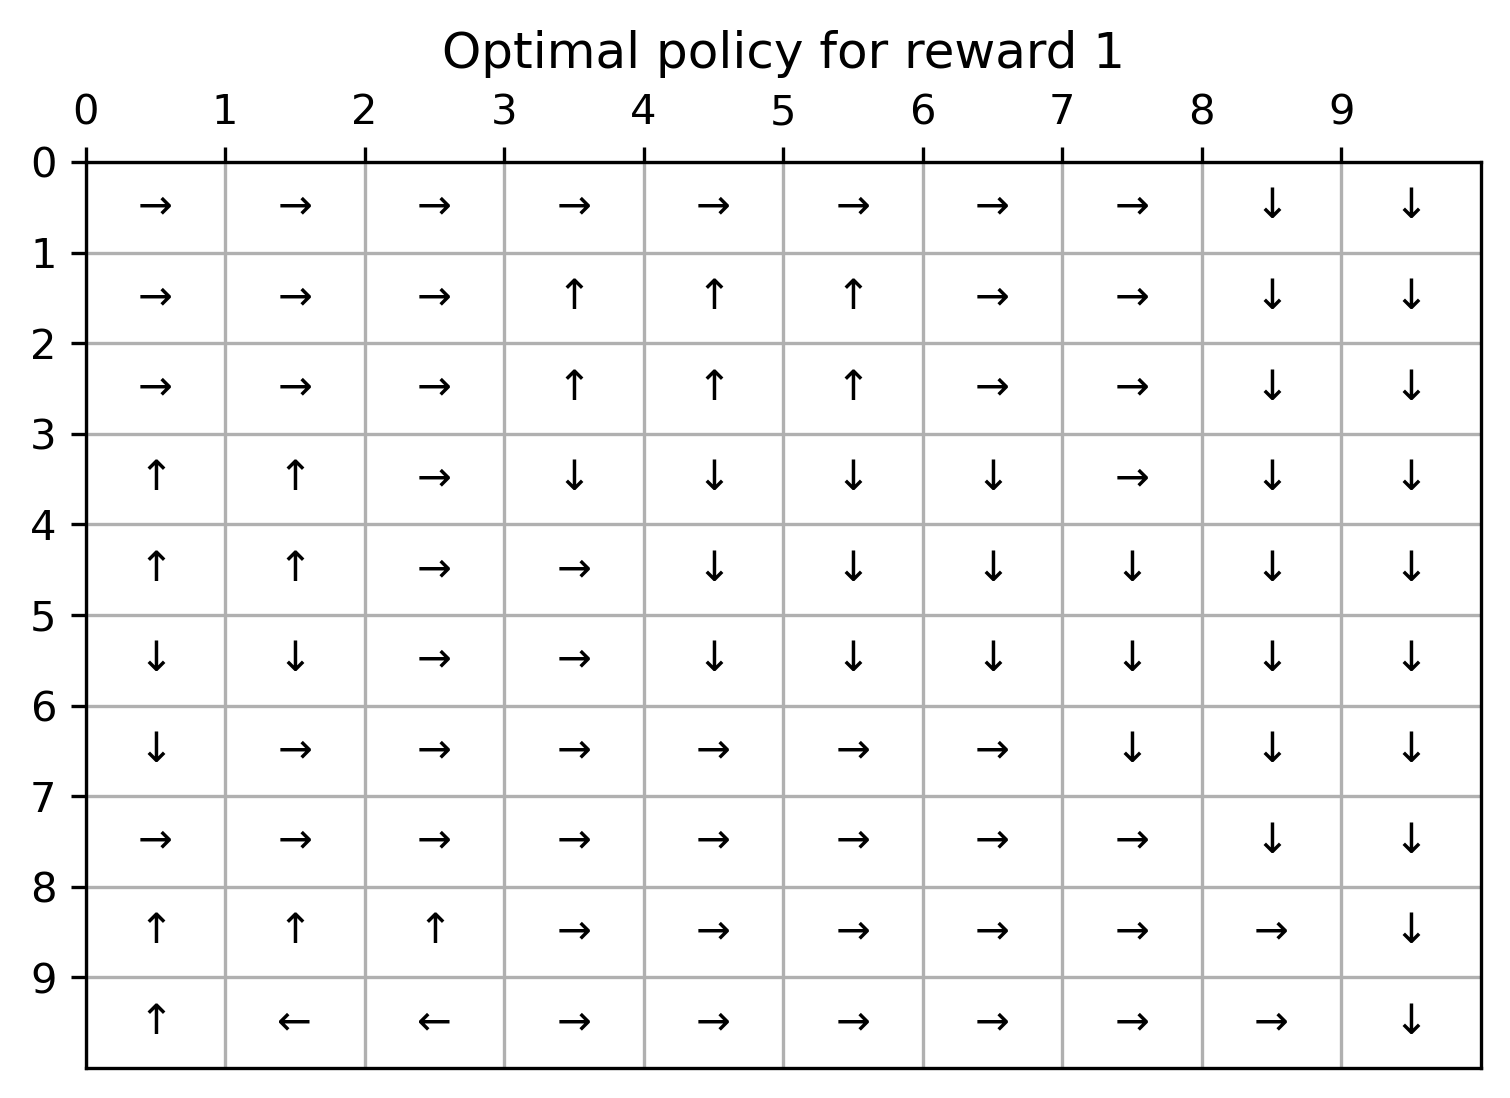
\includegraphics[width=0.49\textwidth]{images/Q1-9/Optimal-policy-for-reward-1.png}
  \caption{Optimal policy for reward 1}
\label{fig: policy1}
\end{figure}

The optimal policy matches our intuition, since the goal of the agent is to maximize the total cumulative reward it can obtain within a finite horizon. For reward function 1, the maximum reward is for state with index 99, the minimum is grouped into three clusters. The action arrows exhibit a pattern to point towards the maximum and away from the minimum.

It is possible for the agent to compute the optimal action by observing the optimal values of the neighbouring states. This is evident when we compare Figure \ref{fig: policy1} with \ref{fig: matrix1}. At each state, the arrow always points towards the neighboring state whose optimal value is highest among all neighbors. Recall the equation to calculate optimal policy:

\begin{equation}
\label{eq: optimal-policy}
     \pi^{*}(s)=\arg \max _{a \in \mathcal{A}} \sum_{s^{\prime} \in \mathcal{S}} \mathcal{P}_{s s^{\prime}}^{a}\left[\mathcal{R}_{s s^{\prime}}^{a}+\gamma V\left(s^{\prime}\right)\right]
\end{equation}

We can see that the optimal policy depends on the optimal values of the neighboring
states, apart from the discount factor, transition matrix and rewards.
\newpage

\section{}\label{sec:6}
Figure \ref{fig: matrix2} shows the optimal values for reward function 2. All but the reward function is the same as \ref{sec:2}.

\begin{figure}[!htb]
\centering
  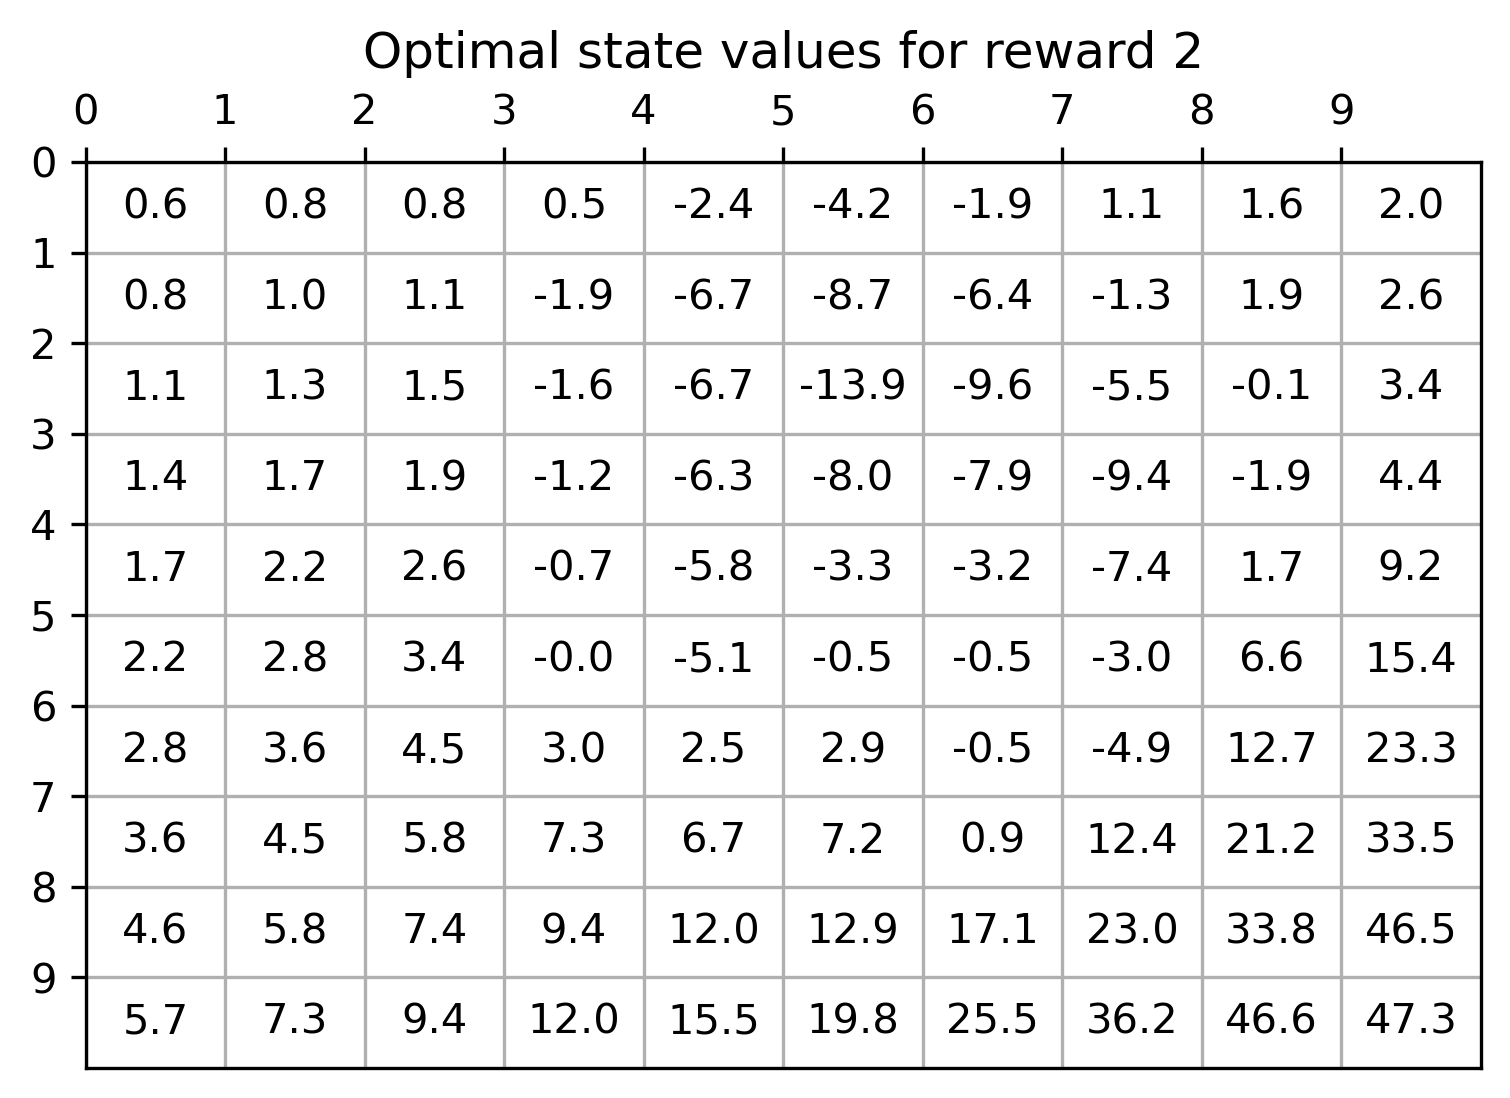
\includegraphics[width=0.49\textwidth]{images/Q1-9/Optimal-state-values-for-reward-2.png}
  \caption{Optimal state values for reward 2}
\label{fig: matrix2}
\end{figure}

\section{}\label{sec:7}
Figure \ref{fig: heatmap3} shows the heatmap of the optimal state value function for reward function 2.

\begin{figure}[!htb]
\centering
  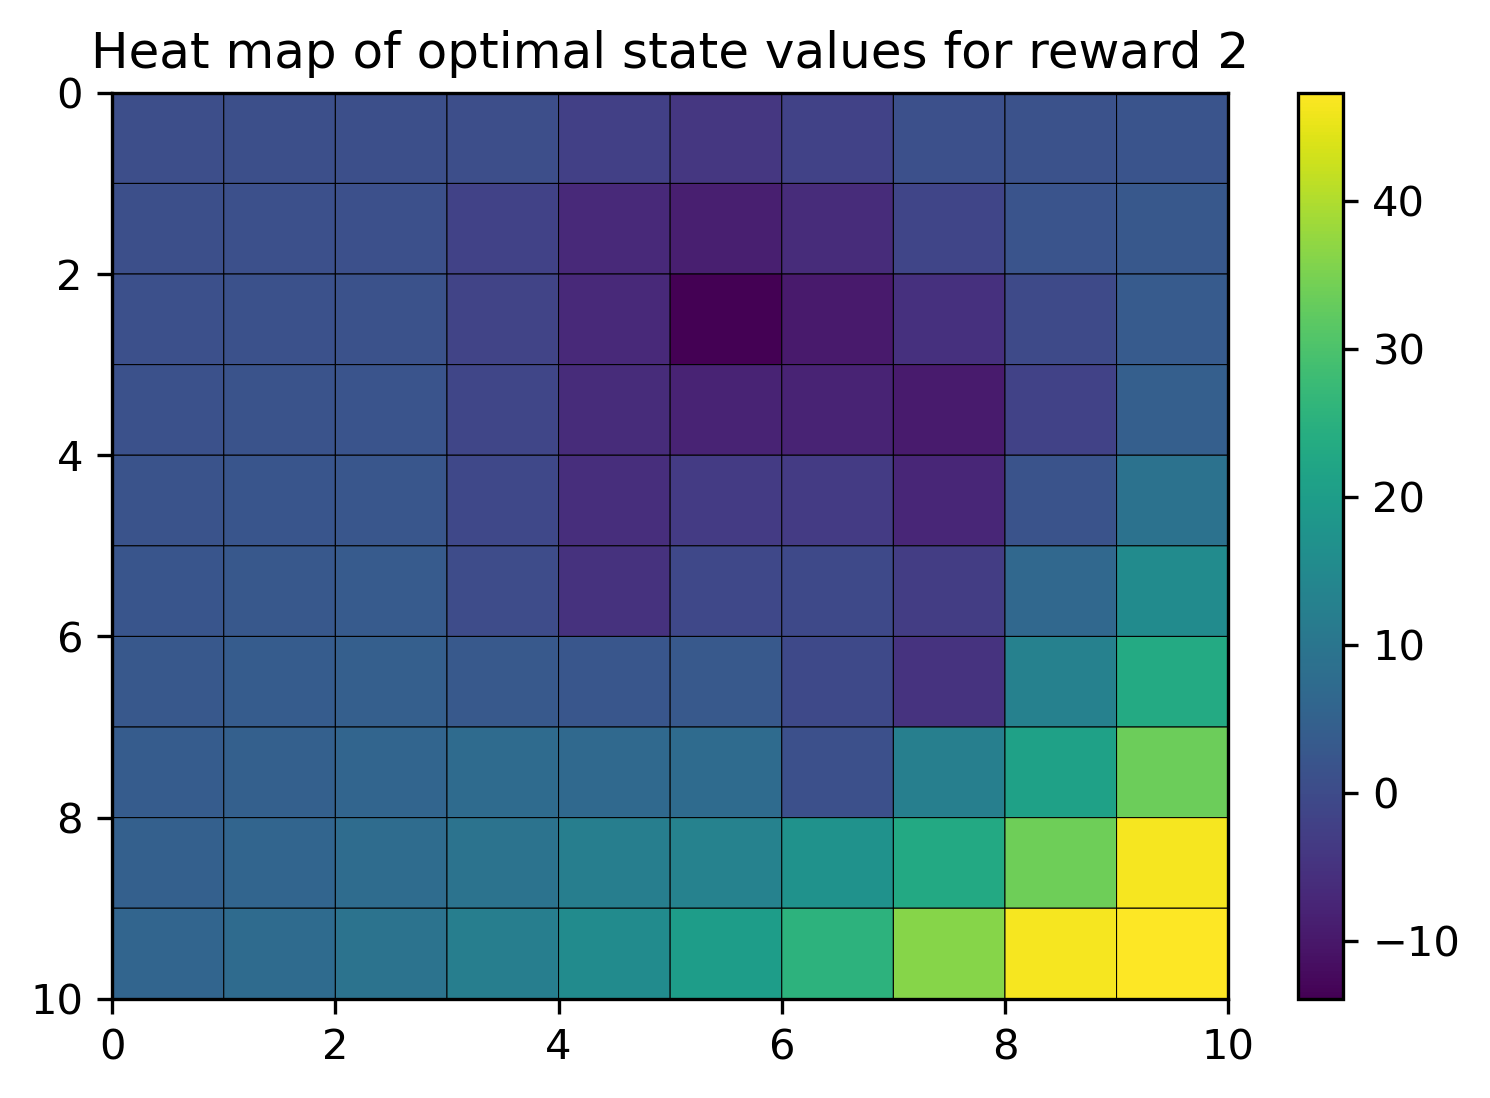
\includegraphics[width=0.49\textwidth]{images/Q1-9/Heat-map-of-optimal-state-values-for-reward-2.png}
  \caption{Heatmap of optimal state value function for reward 2}
\label{fig: heatmap3}
\end{figure}

The heatmap can be explained by similar ideas in \ref{sec:4}. We can see that the state value function largely imitate the reward function in Figure \ref{fig: heatmap1}. The state with index 99 has the largest reward and optimal value, thus also has the brightest color in the heat map. The states represented by the dark colors in the heat map are those with negative rewards. The rest of the states fill in the gradual transition so that the agent would be led towards the targeting state 99 whatever state it starts with.

\section{}\label{sec:8}
Figure \ref{fig: policy2} shows the optimal policy of the agent for reward 2.

\begin{figure}[!htb]
\centering
  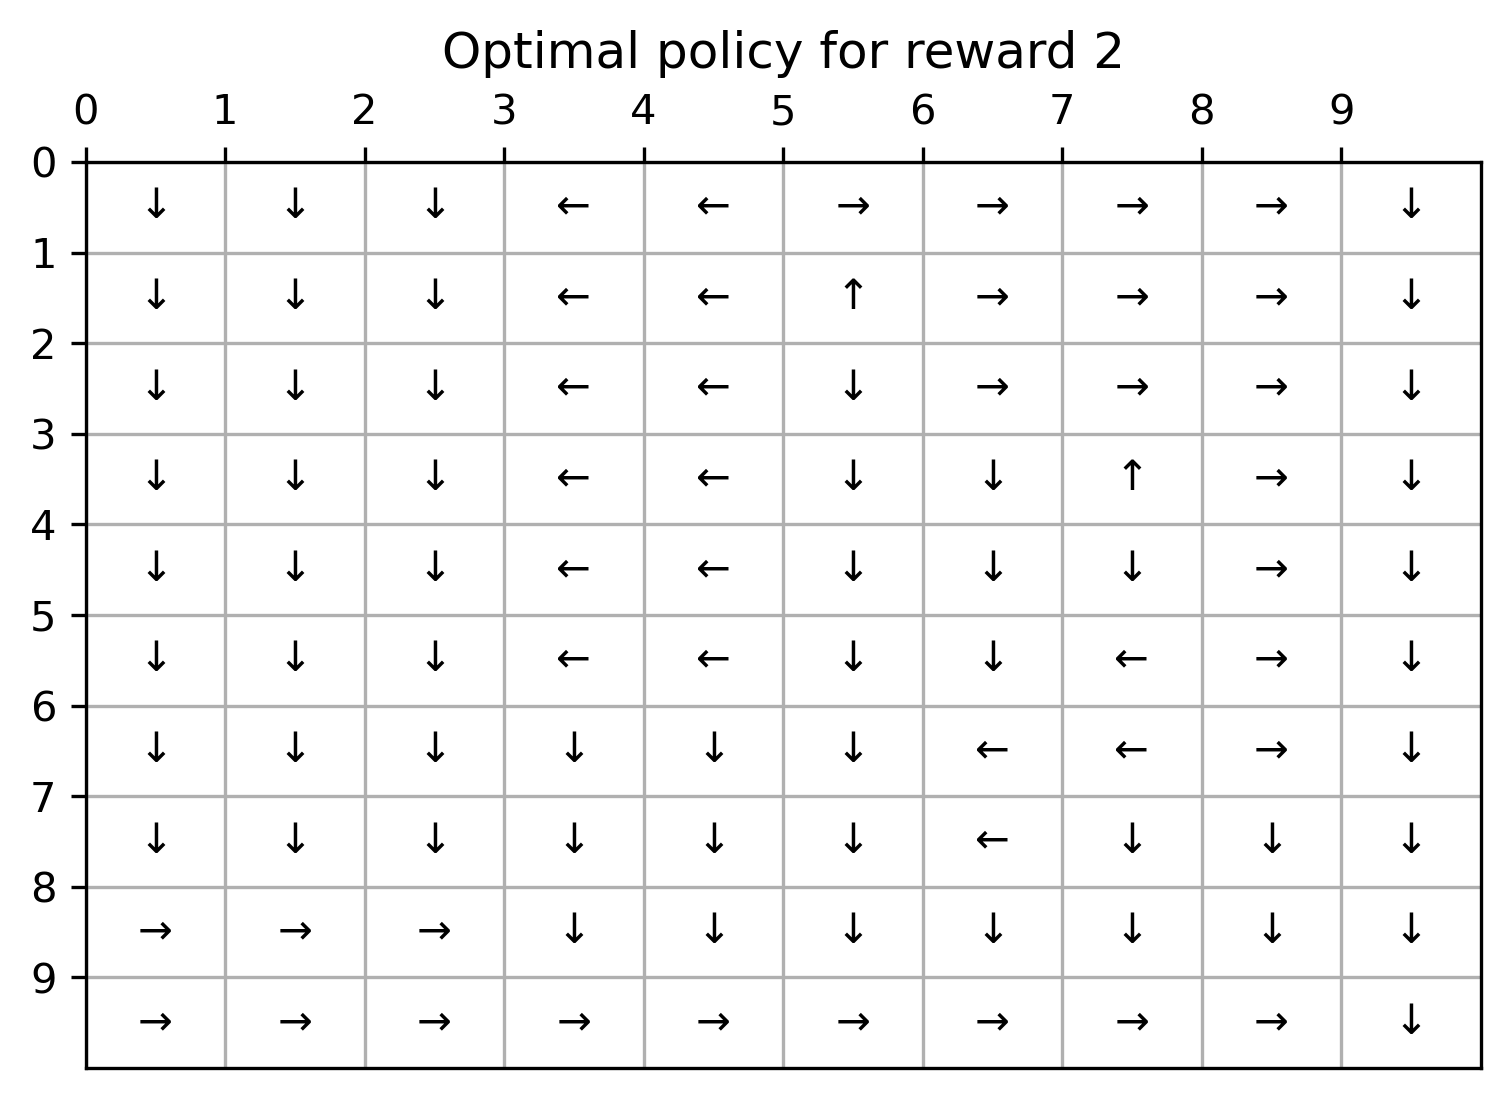
\includegraphics[width=0.49\textwidth]{images/Q1-9/Optimal-policy-for-reward-2.png}
  \caption{Optimal policy for reward 2}
\label{fig: policy2}
\end{figure}

The optimal policy map for reward function 2 also matches our intuition. As we can see from
Figure \ref{fig: heatmap3}, the state with index 53 has the darkest color on the heat map, meaning it has the lowest optimal value. Therefore, in Figure \ref{fig: policy2}, the optimal policy of the states surrounding it exhibits a pattern to move away from it. Moreover, the general policy of all the states is to move towards the state with index 99, which is within our expectation.
\newpage

\section{}\label{sec:9}
Figure \ref{fig: combo1} shows the optimal state value function, its heatmap and optimal policy for reward function 1 and 2 when $w=0.6$. We notice several differences compared to the figures under $w=0.1$:

\begin{itemize}
    \item The optimal values for the maximum and minimum reward state have decreased. The state of the maximum reward only keeps half of the optimal value, while the states with negative reward suffer almost 10 times of value lost. 
    \item The general color of the heatmap, however, is warmer than the previous maps, meaning that the general optimal state value is closer to the maximum. This implies a more distributed state values and a larger uncertainty among the whole state space.
    \item Unlike the optimal policy maps in Figure \ref{fig: policy1} and Figure \ref{fig: policy2} when $w=0.1$, where the optimal policy for most states leads towards state 99, when $w=0.6$, the new optimal policy maps have a higher possibility to lead the agent towards the four corners of the state map as a local optimal result, instead of global optimal result.
    \item We can observe some local optima in the policy plots, where the agent just oscillates between two states, causing a deadlock condition.
\end{itemize}

Intuitively, these differences can be explained by the definition of $w$. $w$ is defined as the possibility that the agent randomly move to one of the four directions due to wind flow. When $w$ changes from 0.1 to 0.6, the agent has a higher possibility to move away from the targeting direction, adding a larger noise to the state value, making the optimal policy more ambiguous.

Theoretically, the differences can also be explained by the exploration versus exploitation dilemma. We can think of $w$ as the probability of exploration. Exploitation is to make the best possible decision by maximizing future reward, while exploration involves taking an immediate sub-optimal action to gather information. Although the sub-optimal action will necessarily involve a reduced amount of reward in the
immediate future, it may allow the agent to learn better strategies that enable policy improvement in the long term. In this case, a high $w$ breaks the balance between exploration and exploitation, making the agent
exploring more sub-optimal actions at each state rather than exploiting knowledge of optimal values reasonably, eventually resulting in a sub-optimal policy.

Based on the analysis above, we choose $w=0.1$ to derive a better optimal policy.

\begin{figure}[!htb]
\centering
  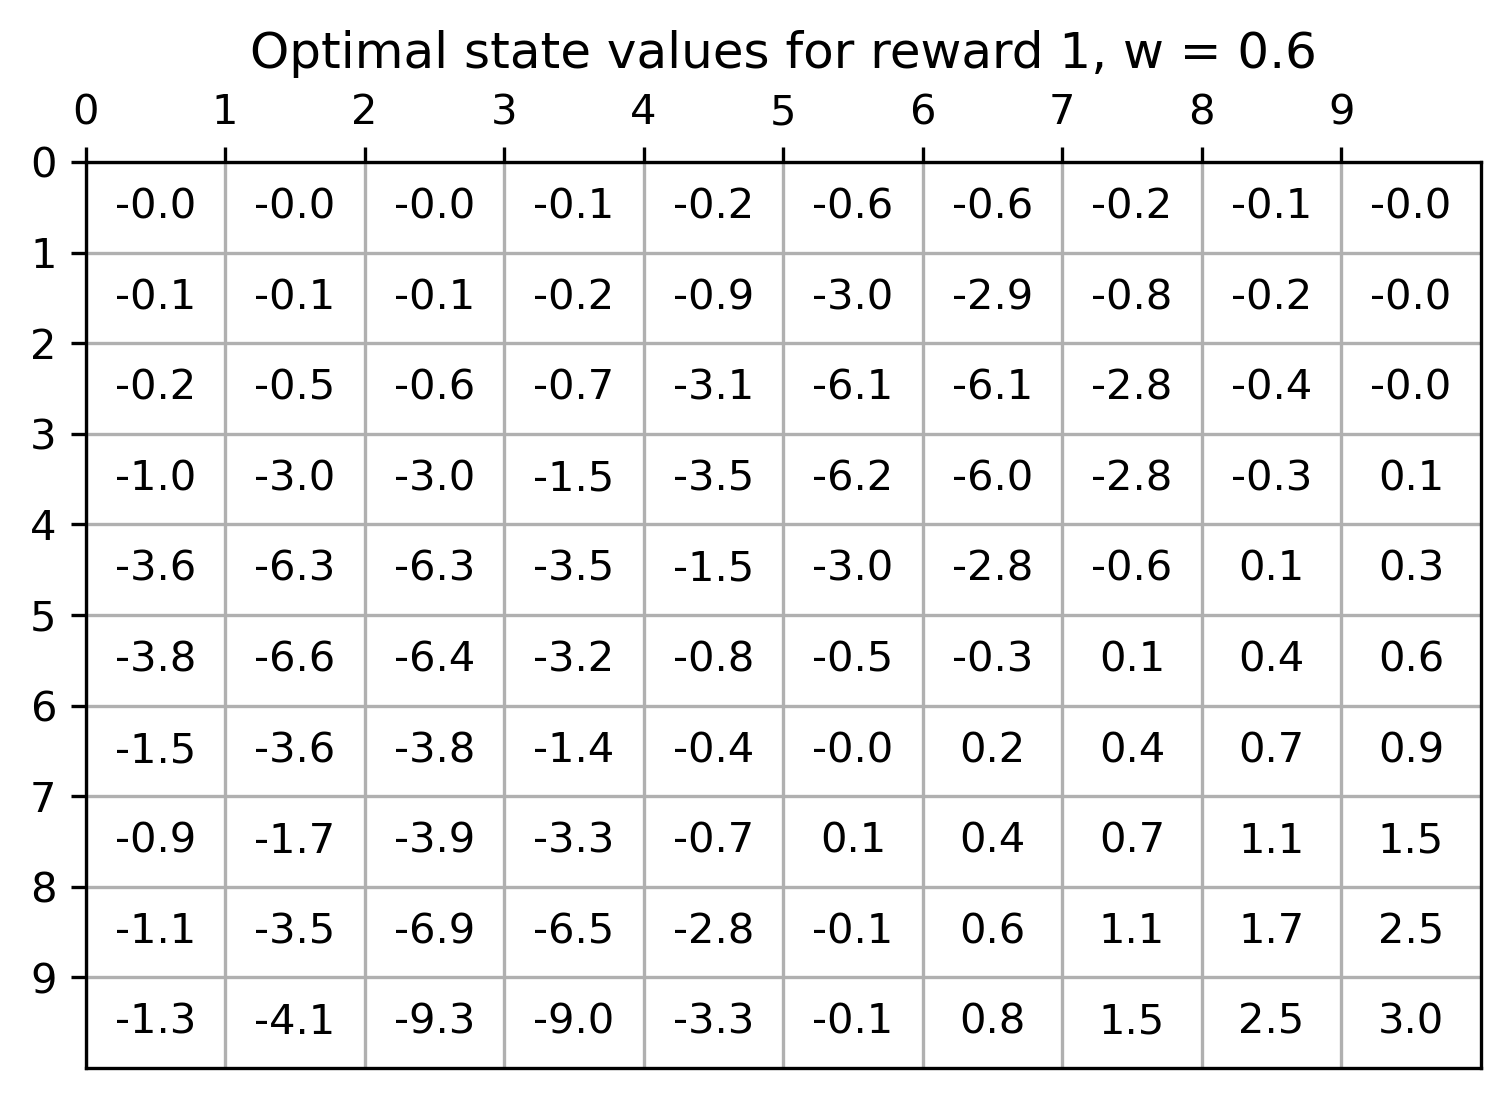
\includegraphics[width=0.49\textwidth]{images/Q9/Optimal-state-values-for-reward-1,-w-=-0.6.png}
  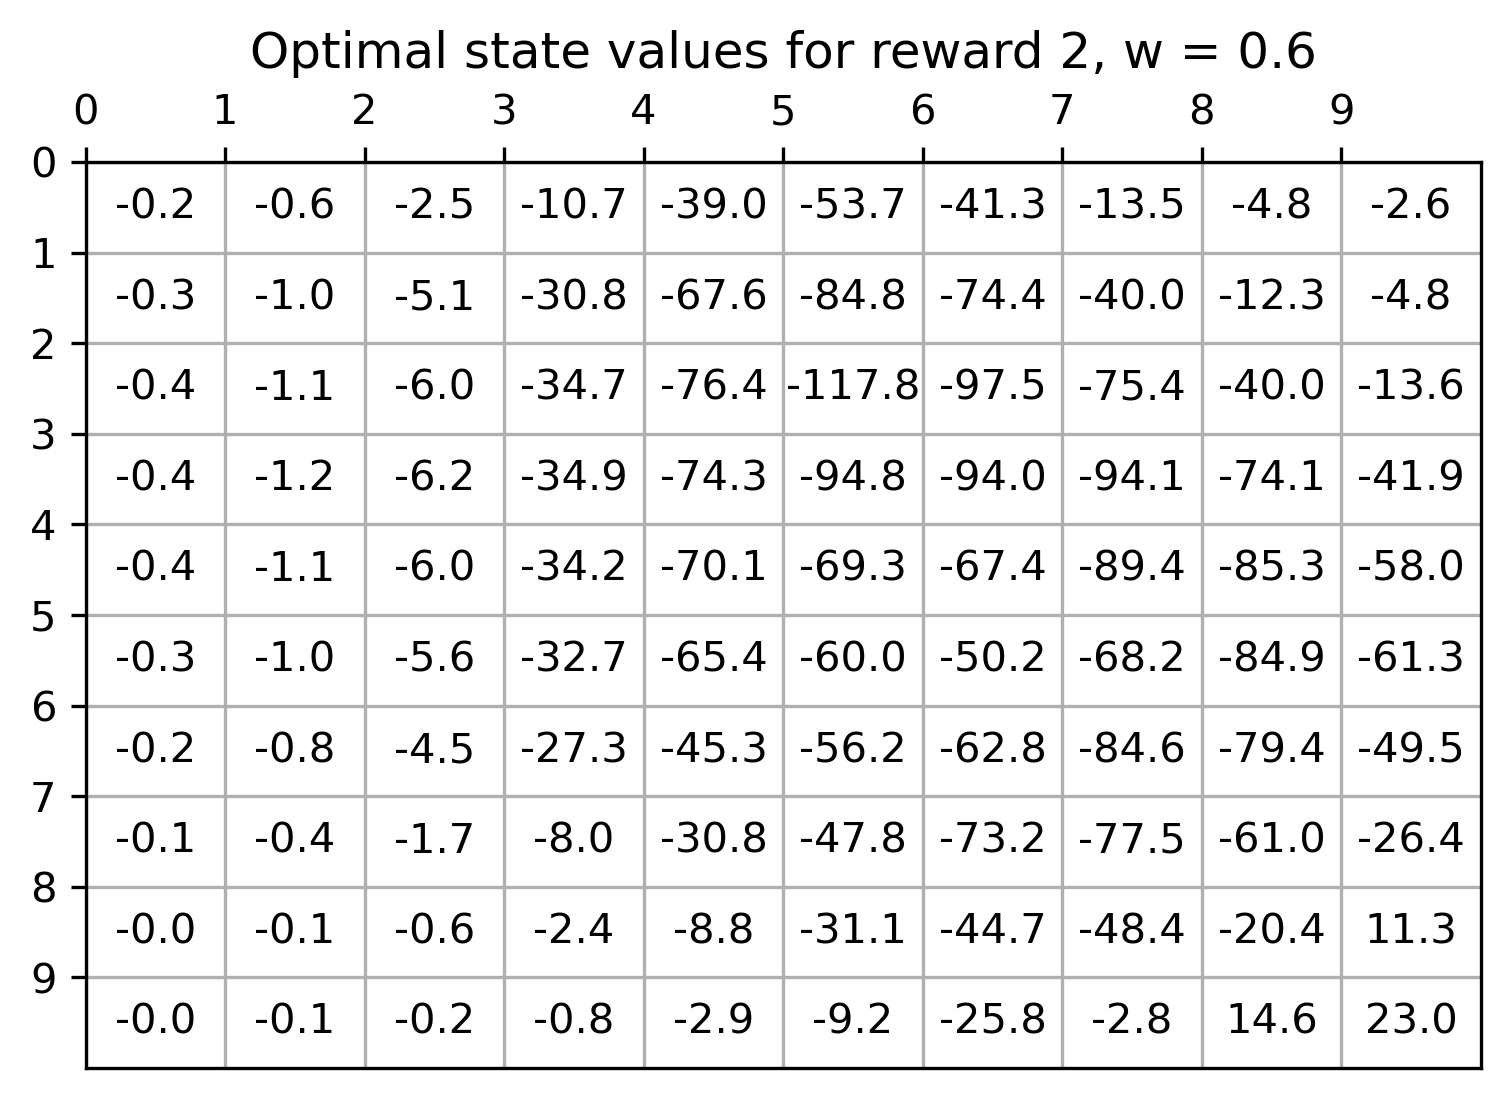
\includegraphics[width=0.49\textwidth]{images/Q9/Optimal-state-values-for-reward-2,-w-=-0.6.png}
  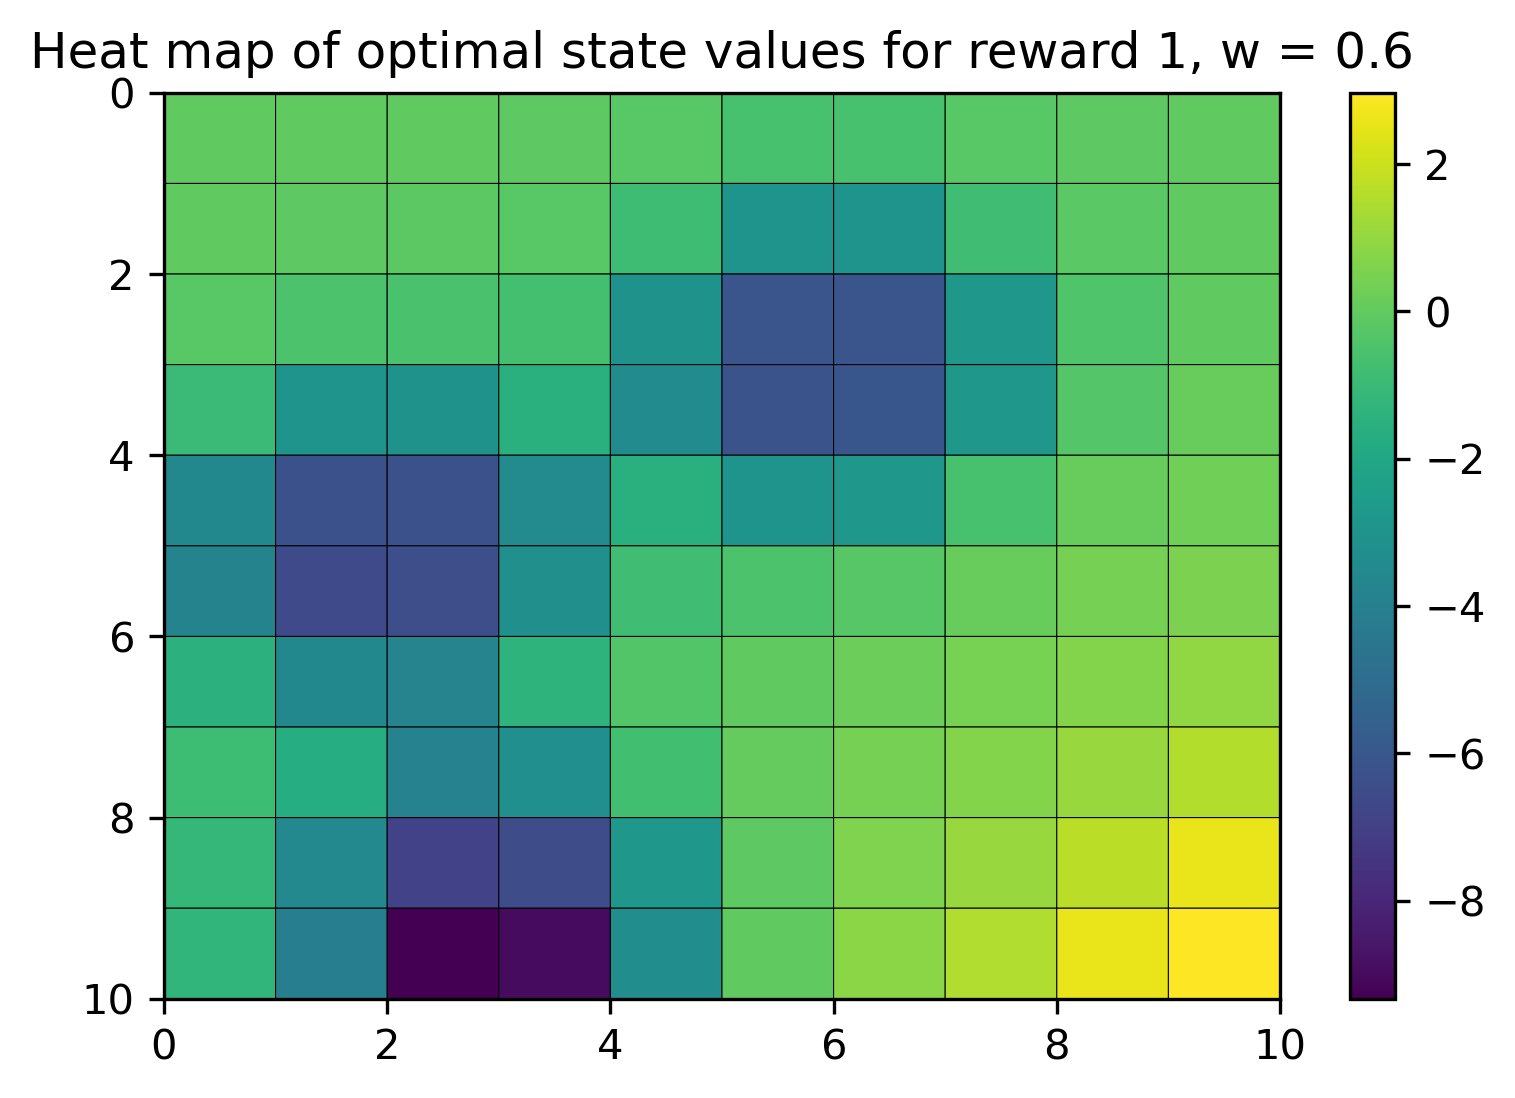
\includegraphics[width=0.49\textwidth]{images/Q9/Heat-map-of-optimal-state-values-for-reward-1,-w-=-0.6.png}
  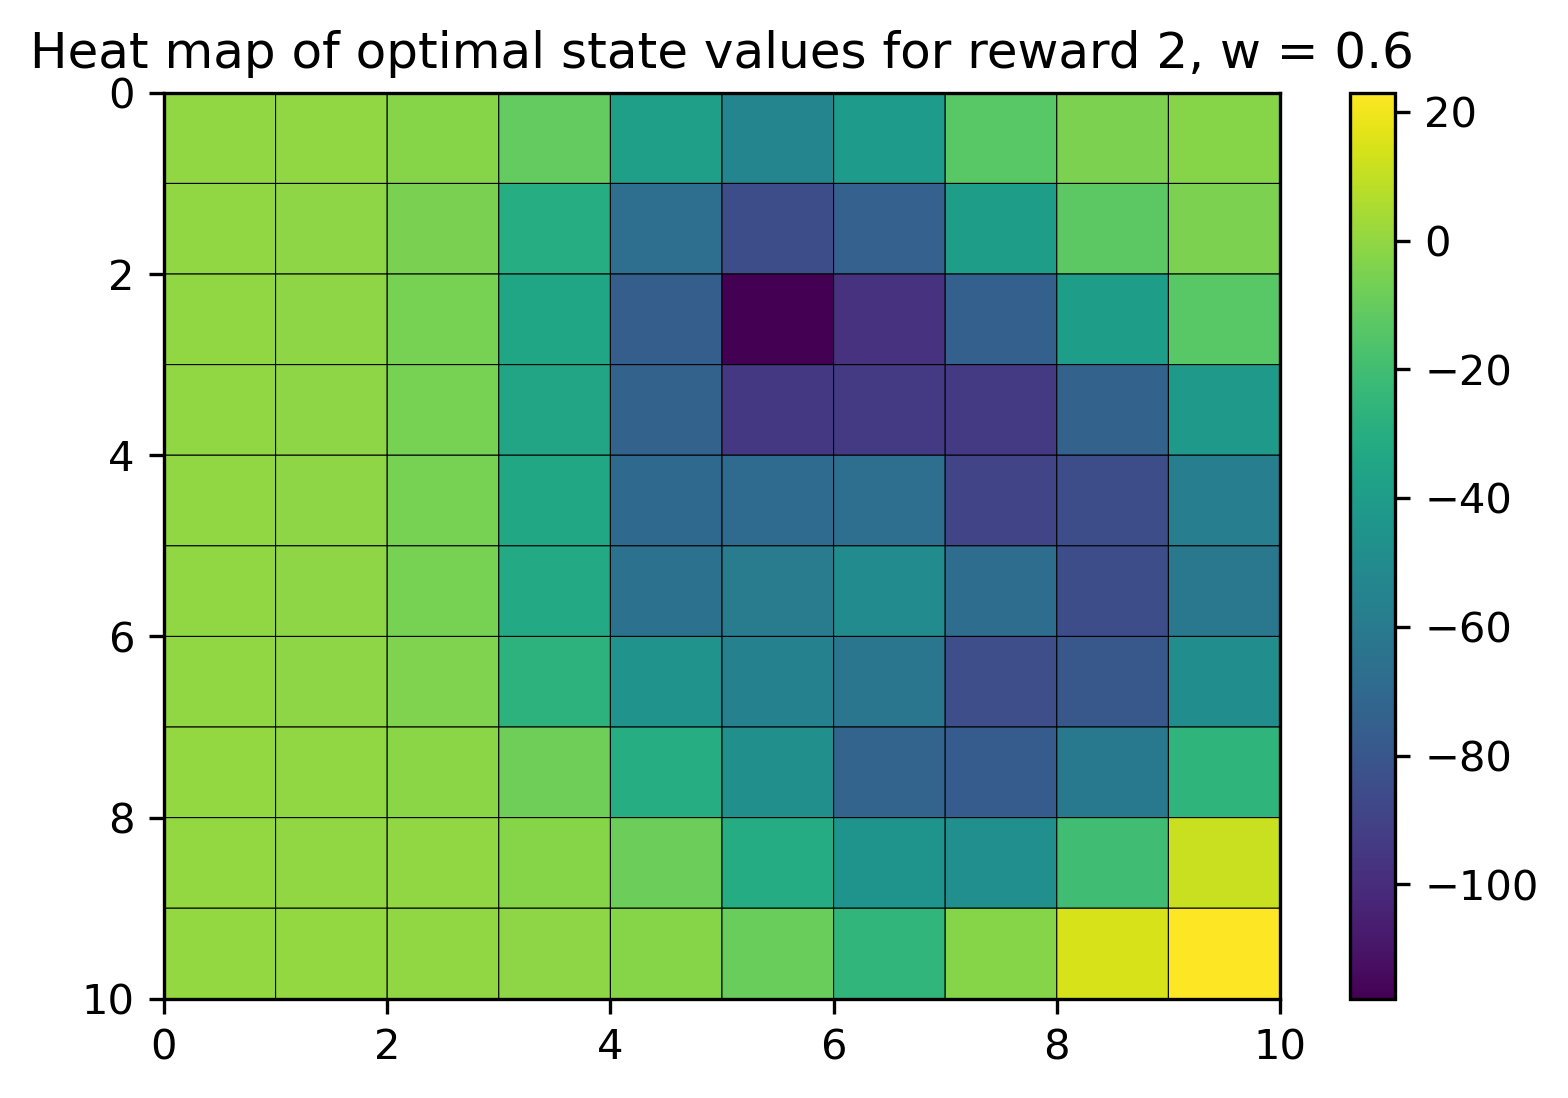
\includegraphics[width=0.49\textwidth]{images/Q9/Heat-map-of-optimal-state-values-for-reward-2,-w-=-0.6.png}
  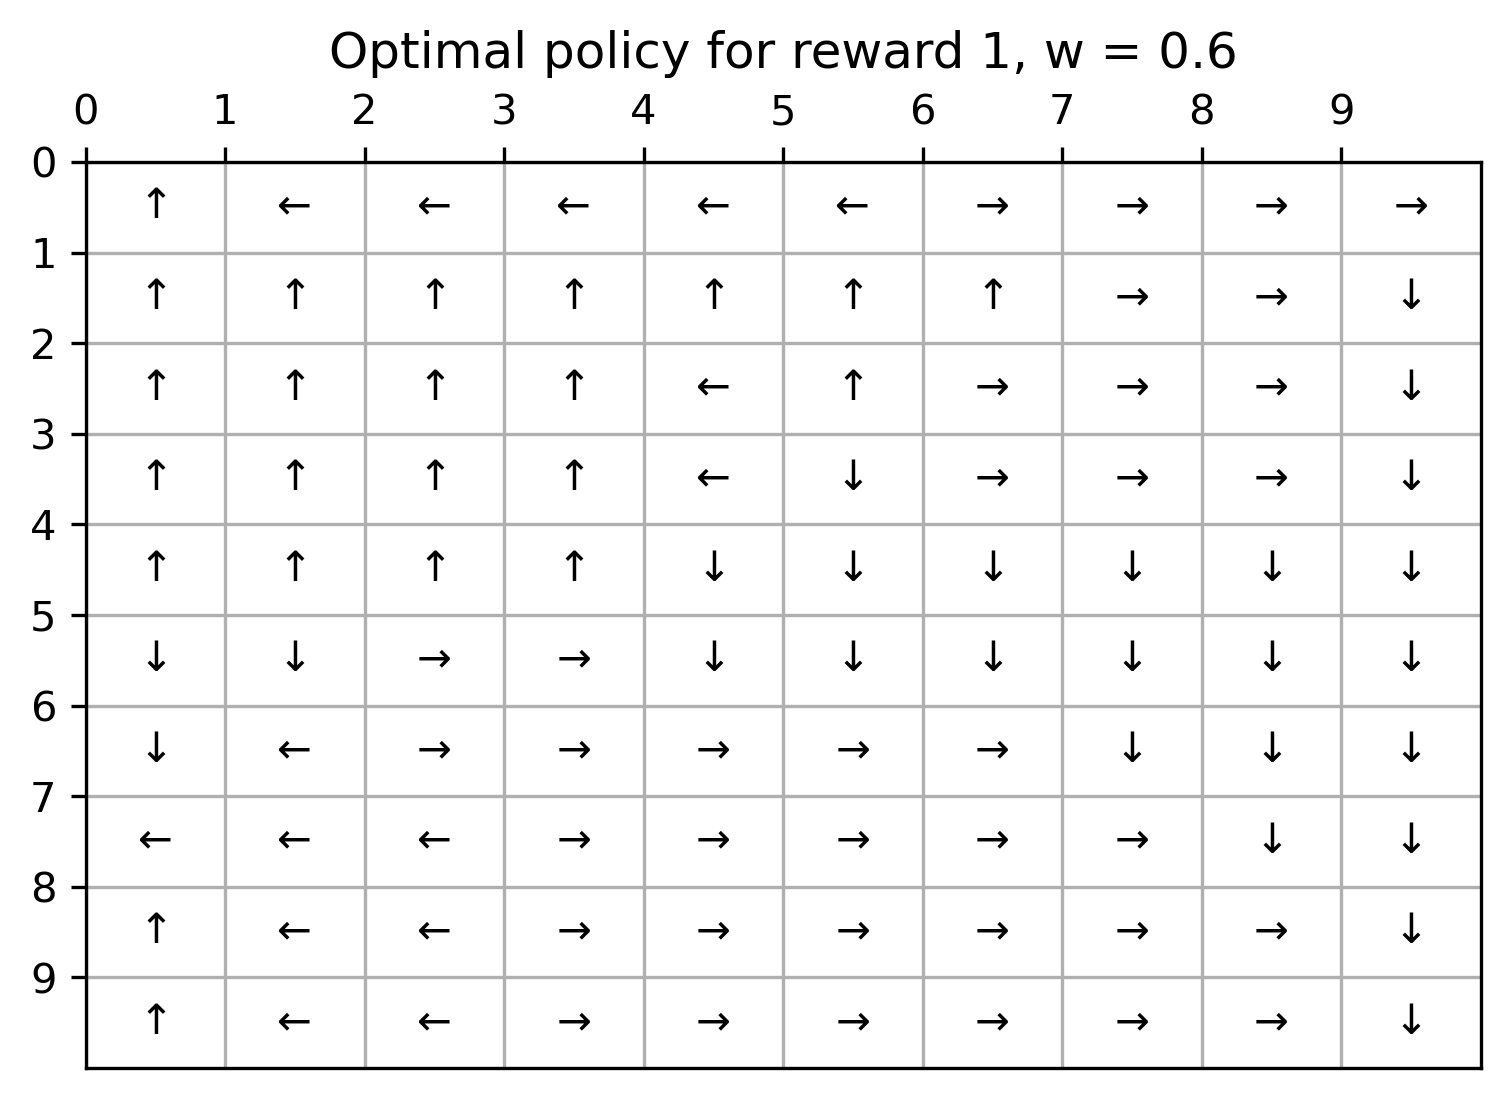
\includegraphics[width=0.49\textwidth]{images/Q9/Optimal-policy-for-reward-1,-w-=-0.6.png}
  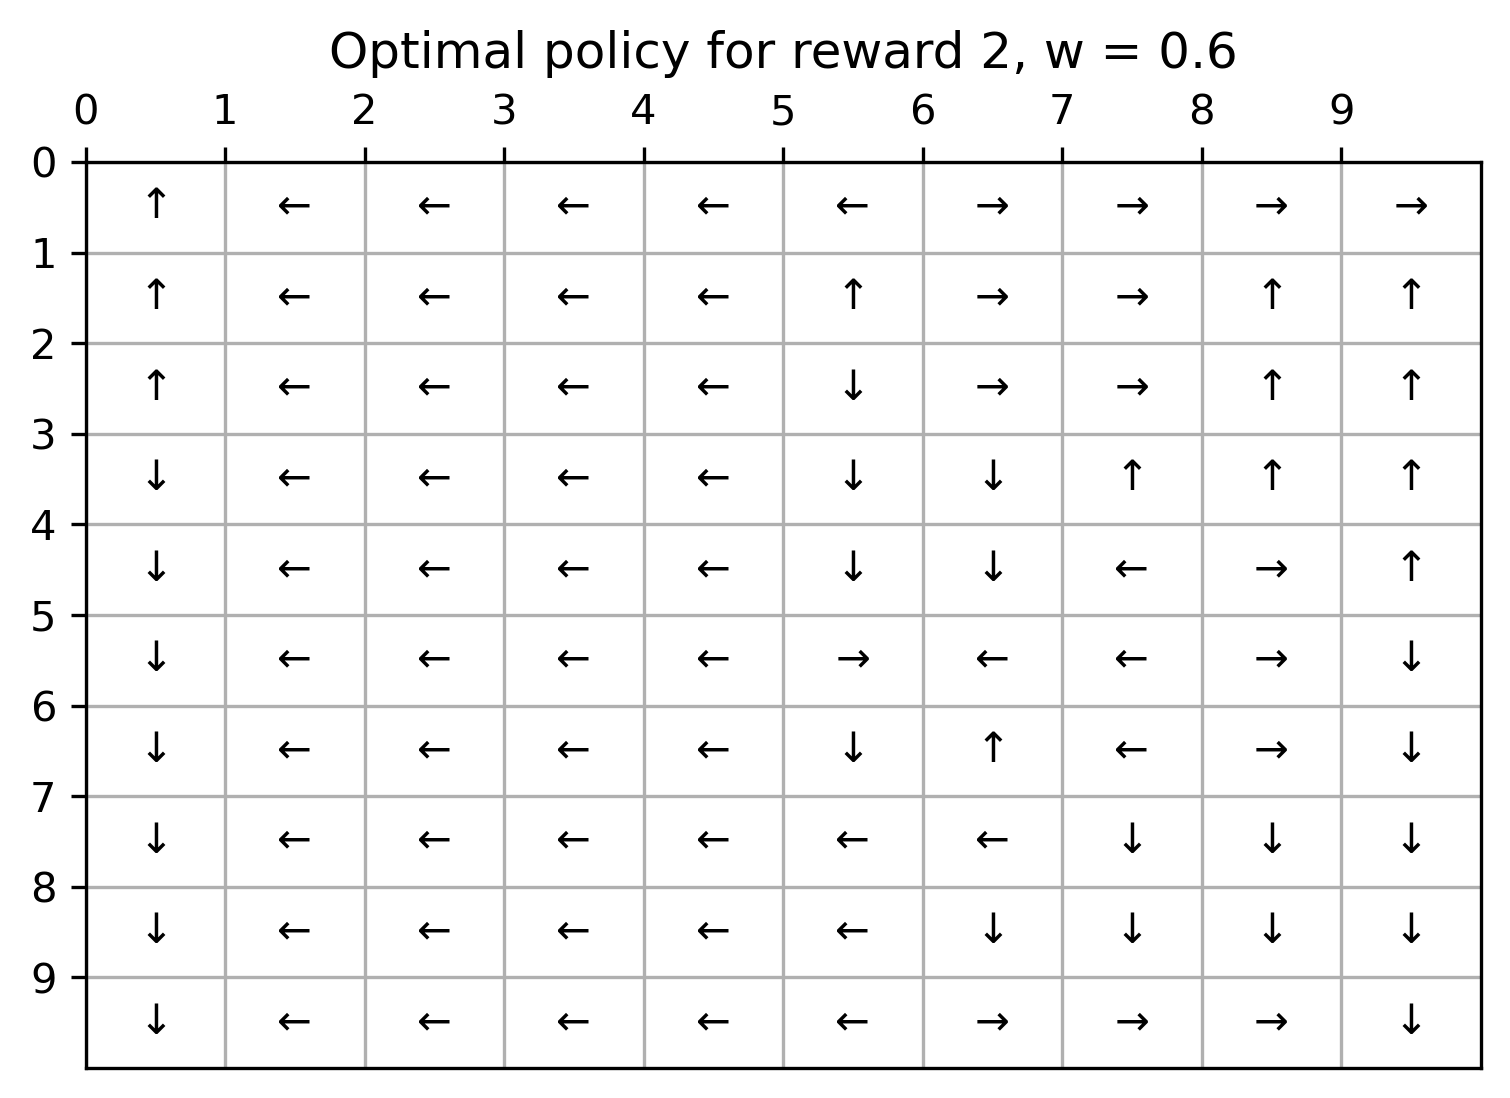
\includegraphics[width=0.49\textwidth]{images/Q9/Optimal-policy-for-reward-2,-w-=-0.6.png}
  \caption{Optimal state values and policy for w = 0.6}
\label{fig: combo1}
\end{figure}
\clearpage

\section{}\label{sec:10}
As described in the question, the LP formulation of the IRL is given by:

\begin{equation}
\label{eq: lp}
    \begin{array}{rcl}
        \operatorname{maximize} & \sum_{i=1}^{|\mathcal{S}|}\left(t_{i}-\lambda u_{i}\right) & \\
        \mathbf{R}, t_{i}, u_{i} \quad \text{subject to} &
        \left[\left(\mathbf{P}_{a_{1}}(i)-\mathbf{P}_{a}(i)\right)\left(\mathbf{I}-\gamma \mathbf{P}_{a_{1}}\right)^{-1} \mathbf{R}\right] \geq t_{i} &
        \forall a \in \mathcal{A} \backslash a_{1}, \forall i \\ & \left(\mathbf{P}_{a_{1}}-\mathbf{P}_{a}\right)\left(\mathbf{I}-\gamma \mathbf{P}_{a_{1}}\right)^{-1} \mathbf{R} \succeq 0 &
        \forall a \in \mathcal{A} \backslash a_{1} \\ &
        -\mathbf{u} \preceq \mathbf{R} \preceq \mathbf{u} \\ & \left|\mathbf{R}_{i}\right| \leq R_{\max } &
        i=1,2,\cdots,|\mathcal{S}|
    \end{array}
\end{equation}

For the ease of implementation, we recast Equation \ref{eq: lp} into Equation \ref{eq: lp-matrix} using block matrices:

\begin{equation}
\label{eq: lp-matrix}
    \begin{array}{rcl}
        \operatorname{maximize} & \mathbf{c}^{T} \mathbf{x} & \\
        \mathbf{x} \quad \text{subject to} &
        \mathbf{D x} \preceq \mathbf{b} &
        \forall a \in \mathcal{A} \backslash a_{1}
    \end{array}
\end{equation}

Therefore, we can derive the matrix entries in Equation \ref{eq: lp-matrix} as follows:

\begin{equation}
\label{eq: c}
    \mathbf{c}=\left(\begin{array}{c}\mathbf{I} \\ -\lambda \cdot \mathbf{I} \\ 0\end{array}\right) \in \mathbb{R}^{3|\mathcal{S}| \times|\mathcal{S}|}
\end{equation}

\begin{equation}
\label{eq: x}
    \mathbf{x}=\left(\begin{array}{c}\mathbf{t} \\ \mathbf{u} \\ \mathbf{R}\end{array}\right) \in \mathbb{R}^{3|\mathcal{S}| \times 1}, \text { where } \mathbf{t}=\left(\begin{array}{c}t_{1} \\ t_{2} \\ \vdots \\ t_{|\mathcal{S}|}\end{array}\right), \mathbf{u}=\left(\begin{array}{c}u_{1} \\ u_{2} \\ \vdots \\ u_{|\mathcal{S}|}\end{array}\right), \mathbf{R}_{i}=\mathbf{R}\left(s_{i}\right)
\end{equation}

\begin{equation}
\label{eq: d}
    \mathbf{D}=\left(\begin{array}{ccc}\mathbf{I} & 0 & -\left(\mathbf{P}_{a_{1}}-\mathbf{P}_{a}\right)\left(\mathbf{I}-\gamma \mathbf{P}_{a_{1}}\right)^{-1} \\ 0 & 0 & -\left(\mathbf{P}_{a_{1}}-\mathbf{P}_{a}\right)\left(\mathbf{I}-\gamma \mathbf{P}_{a_{1}}\right)^{-1} \\ 0 & -\mathbf{I} & -\mathbf{I} \\ 0 & -\mathbf{I} & \mathbf{I} \\ 0 & 0 & \mathbf{I} \\ 0 & 0 & -\mathbf{I}\end{array}\right) \in \mathbb{R}^{10|\mathcal{S}| \times 3|\mathcal{S}|}, \forall a \in \mathcal{A} \backslash a_{1}
\end{equation}

\begin{equation}
\label{eq: b}
    \mathbf{b}=\left(\begin{array}{c}0 \\ 0 \\ 0 \\ 0 \\ R_{\max } \cdot \mathbb{1} \\ R_{\max } \cdot \mathbb{1}\end{array}\right) \in \mathbb{R}^{6|\mathcal{S}| \times 1}
\end{equation}

\newpage

\section{}\label{sec:11}
We first create the function \verb"construct_lp_matrices" to construct block matrices used in the LP formulation. We then create \verb"solve_lp" which uses the LP solvers from \verb"cvxopt" to solve the LP problem and obtain the predicted reward function. We put the reward back to function \verb"value_iteration" to get the optimal action of the agent $O_{A}(s)$.

The accuracy of the IRL algorithm is given as:

\begin{equation}
\label{eq: accuracy}
    Accuracy=\frac{\sum_{s \in S} m(s)}{|S|}, \quad m(s)=\left\{\begin{array}{l}1, O_{A}(s)=O_{E}(s) \\ 0, \text { else }\end{array}\right.
\end{equation}

We use the optimal policy extracted in \ref{sec:5} as the optimal action of the expert $O_{E}(s)$. In order to find the $\lambda$ that has the best performance for IRL algorithm, we sweep $\lambda$ from 0 to 5 to get 500 evenly spaced values. The relationship between $\lambda$ and the accuracy score is shown in Figure \ref{fig: accuracy1}. We can see that the accuracy of the IRL algorithm first increases with $\lambda$ and reaches a global optimum. It then remains largely stable until a sudden drop when $\lambda \approx 3.7$.

\begin{figure}[!htb]
\centering
  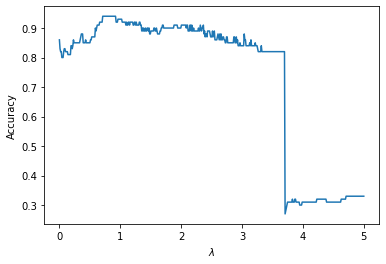
\includegraphics[width=0.49\textwidth]{images/Q11/Accuracy.png}
  \caption{Accuracy of IRL algorithm for reward 1}
\label{fig: accuracy1}
\end{figure}

\section{}\label{sec:12}
From Figure \ref{eq: accuracy} we can derive that, when $\lambda_{\max }^{(1)} \approx 0.71$, the accuracy score can reach up to 95\%.